\documentclass[11pt]{article}

\usepackage{amssymb,amsmath,amsfonts,mathtools,eurosym,geometry,ulem,graphicx,caption,color,setspace,sectsty,comment,caption,pdflscape,subfigure,array,xr,paralist}

\newcommand\myeq{\stackrel{\mathclap{\normalfont\mbox{\tiny ind}}}{\sim}}

\usepackage[hidelinks]{hyperref}
\usepackage{natbib}
\usepackage{enumitem}
\setlist{itemsep=0pt}
\usepackage[bottom]{footmisc}

\newcommand*{\footcite}[1]{\cite{#1}}

\externalcitedocument{/Users/asheth/Library/CloudStorage/OneDrive-iCapitalNetwork/GMAM/literature/litreview/LitReview}

\normalem

\onehalfspacing
\newtheorem{theorem}{Theorem}
\newtheorem{corollary}[theorem]{Corollary}
\newtheorem{proposition}{Proposition}
\newenvironment{proof}[1][Proof]{\noindent\textbf{#1.} }{\ \rule{0.5em}{0.5em}}

\newtheorem{hyp}{Hypothesis}
\newtheorem{subhyp}{Hypothesis}[hyp]
\renewcommand{\thesubhyp}{\thehyp\alph{subhyp}}

\newcommand{\red}[1]{{\color{red} #1}}
\newcommand{\blue}[1]{{\color{blue} #1}}

\newcolumntype{L}[1]{>{\raggedright\let\newline\\arraybackslash\hspace{0pt}}m{#1}}
\newcolumntype{C}[1]{>{\centering\let\newline\\arraybackslash\hspace{0pt}}m{#1}}
\newcolumntype{R}[1]{>{\raggedleft\let\newline\\arraybackslash\hspace{0pt}}m{#1}}

\geometry{left=1.0in,right=1.0in,top=1.0in,bottom=1.0in}

\begin{document}

%\begin{titlepage}
\title{Bayesian Estimation of Private Equity Returns}
\author{iCapital Quant Research Team}
\date{\today}


\maketitle

\newpage

\begin{abstract}
\noindent We develop a methodology to estimate a time series of private equity returns based on returns as reported by general partners using a hierarchical Bayesian model.  We do this at the fund level. Our methodology incorporates a moving-average process to manage the problem of stale NAVs and returns smoothing. In addition, we use a spike-and-slab regression to determine which factors drive a specific funds returns. We use a unique dataset of fund-level returns provided to us by the funds themselves. This process also allows us to easily analyze the returns of a portfolio consisting of public and private securities. \\

\noindent\textbf{Keywords:} Bayesian filtering, private equity, returns generation\\

\vspace{0in}

%\noindent\textbf{JEL Codes:} key1, key2, key3\\
\end{abstract}

\newpage

%\tableofcontents
%
%\newpage

%\begin{figure}[!ht]
%	\centering
%	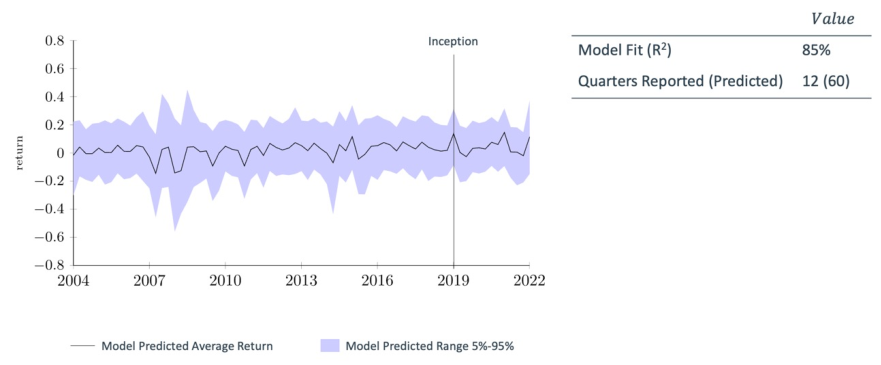
\includegraphics[width=475pt]{results.pdf}
%	\caption{An example of a fund’s returns as generated by GMAM 3.0. The fund was incepted in 2019, and backcasted to 2004 using a hierarchical Bayesian technique. De-smoothed returns were generated, and re-smoothed again to reflect what the actual fund returns would look like. This helps investors to pair the fund with a portfolio of publicly available securities.}
%\end{figure}


%\begin{abstract}
%\noindent We develop a methodology to estimate a time series of private equity returns based on returns as reported by general partners using a hierarchical Bayesian model.  We do this at the fund level. Our methodology incorporates a moving-average process to manage the problem of stale NAVs and returns smoothing. In addition, we use a spike-and-slab regression to determine which factors drive a specific funds returns. We use a unique dataset of fund-level returns provided to us by General Partners. This process also allows us to easily analyze the returns of a portfolio consisting of public and private securities. \\
%\noindent\textbf{Keywords:} Bayesian filtering, private equity, returns generation\\
%\vspace{0in}\\
%\noindent\textbf{JEL Codes:} key1, key2, key3\\

%\bigskip
%\end{abstract}

\setcounter{page}{0}
\thispagestyle{empty}
%\end{titlepage}





%\doublespacing


\section{Introduction} 
\label{sec:introduction}

Data from past years suggest that alternative investments such as private equity and hedge funds are trending upwards. For instance, Bain \& Company  valued\footnote{Source:\href{https://www.bain.com/insights/topics/global-private-equity-report/}{https://www.bain.com/insights/topics/global-private-equity-report/}} private equity  buyout deals for 2022 at \$654 billion globally. This was the second-highest valuation since 2008 and brought total deal volume to \$2.4 trillion\footnote{Source:\href{https://www.mckinsey.com/industries/private-equity-and-principal-investors/our-insights/mckinseys-private-markets-annual-review/}{https://www.mckinsey.com/industries/private-equity-and-principal-investors/our-insights/mckinseys-private-markets-annual-review/}}. On the investor side, SEC rules defining the term `accredited investor', have recently broadened to include ``individual investors that have the knowledge and expertise to participate in [financial] markets.'' One no longer needs to pass the income requirement. \\

In addition, firms like iCapital have hastened the market expansion and liquidity of alternative investments such as private equity and made it a viable option for accredited investors and private wealth funds\footnote{Source:\href{https://icapital.com/insights/practice-management/untapped-potential-alternative-investments-and-the-wealth-management-channel/}{https://icapital.com/insights/practice-management/untapped-potential-alternative-investments-and-the-wealth-management-channel/}}. While pension funds and endowments have had access to such investments for decades (see, for example, \cite{Takahashi2002}), this is the first time in history that they are poised to become this widespread. With all this, it becomes increasingly pertinent to have good tools that enable investors to analyze portfolios of alternative investments combined with traditional public investments like stocks and bonds. It is also important that such tools have a solid grounding in asset pricing theory. \\

Our model promises to do all of that. \\

A significant limitation for the analysis for PE and other alternative asset returns is the lack of availability of performance metrics based on actual transactions since alts are largely exempt from public disclosure requirements. This limitation impedes the process of optimal wealth allocation since this process requires data on the risk, return, and covariance of asset classes. In liquid markets, these can be calculated via historical return data. So how does one optimally combine such assets with publicly available investment opportunities? \\

iCapital Network’s attempts to solve this problem and others associated with returns on illiquid, alternative investments via our Generalized Multi-Asset Model version 3.0 (henceforth, GMAM 3). GMAM 3 is a returns-generating model that uses hierarchical Bayesian modeling techniques to generate economically significant returns for any single fund that trades on iCapital’s marketplace. This model helps to educate investors on whether or not a particular fund is suitable for them, based on their investment needs and risk preferences. \\

There are several unique aspects of the model, and this technical manual explains the motivation behind the choices made as well as their economic rationale.

\subsection{Why Bayesian?}
Bayesian techniques offer a more robust and flexible approach to capture the complex dynamics of private equity returns due to their ability to:
\begin{itemize}
\setlist{itemsep=0pt}
	\item incorporate prior knowledge,
	\item handle limited data,
	\item account for iliquidity, and
	\item update estimates as new information becomes available.
\end{itemize}

They allow one to incorporate prior beliefs or information about specific funds into the estimation of returns. This prior information is leveraged to handle limited data. These techniques also allow for the incorporation of uncertainty into the return estimates by providing probability distributions rather than point estimates. They provide a framework that aligns well with the unique characteristics of private equity investments, allowing for more accurate and informed returns estimation. \\

For example, it well-known in the academic finance literature that for private equity (henceforth, PE) returns there is a dearth of performance metrics based on actual transactions (\cite{Kaplan2005}). Also, the available time series data often relies on non-market valuations or multiyear internal rates of return (IRR) that are segmented by the vintage years of the funds which further complicates the calculation. For investors seeking to optimally allocate their wealth across public securities and private equity, this is a significant barrier. For instance, even a simple Markowitz-style (\cite{markowitz}) mean-variance optimization requires a sufficiently long history of returns which is unavailable in the case of PE. \\

As mentioned above, one commonly used metric in the PE world to gauge a fund’s performance is the IRR. It provides a convenient way by which to compare and benchmark various funds. Furthermore, it is an easy way to account for the timing and magnitude of cash flows since PE investments are typically illiquid and longer investment horizons. And finally, it helps investors assess the risk of a fund. \\

While these are good reasons to use the IRR, there are numerous measurement concerns related to it. One implicit assumption when calculating IRRs is that the cash proceeds will be reinvested to achieve a particular return. This assumption does not coincide with the reality of cash flow distributions by PE. For example, if a PE fund reports a 50\% IRR and has returned cash early in its life, the assumption is that the cash will be reinvested at 50\%. However, it is unlikely that the fund will find such an investment opportunity every time cash is distributed. \\

Furthermore, IRR can distort management incentives, upwardly bias performance measures, and misrepresent volatility estimates (\cite{Phalippou2008}). As stated in \cite{Sorensen2013}, ``The IRR may not exist, and it may not be unique.'' Even though the Modified IRR (MIRR) largely tackles some well-known pitfalls of IRR, its practical implementation in a private partnership is not obvious. \\

GMAM 3, on the other hand, uses time-weighted returns. 
\begin{equation}
	y_t = \frac{NAV_t + Distributions_t}{NAV_{t-1} + Contributions_t}
\end{equation}

Though these have their own caveats\footnote{They may not fully capture the complexities of private equity investments, such as the strategic timing of cash flows and the long-term, illiquid nature of these assets.}, they also have their strengths. For instance, this method of calculation accounts for the contributions and distributions, as well as their timing. Also, it allows for a more standardized comparison of performance across different investment vehicles and asset classes. This applies especially to investors who wish to combine PE with publicly available investments. And finally, it is a widely understood and commonly used method in the broader investment industry. Its use in measuring PE performance can facilitate understanding and communication about fund performance, especially for stakeholders more familiar with traditional investment vehicles. \\

One of the strengths of the model’s Bayesian estimation process provides measures of uncertainty around the estimated returns, and this allows the user to decide for themselves the degree to which they can rely on these estimated, time-weighed returns.

\section{The Model}
At its core, the model predicts fund returns from factor returns. The essence of the GMAM 3 returns-generating process can be modeled as:
\begin{equation}
	x_{i,t} = f^{\prime}_t \beta_{i,t} + r_t^f + \varepsilon_{i,t}
\end{equation}

where $f_t$ is a length $K$ vector of factor returns including an intercept dummy, $\beta_{i,t}$  is a $K \times 1$ matrix of exposures, $x_{i,t}$ is the predicted return, $r_t^f$ is the risk-free rate of return, and $\varepsilon_{i,t}$ is the error. The subscripts here are for an individual fund ($i$) for a given period ($t$). Henceforth, assume that all measures are for an individual fund, and so the $i$-subscript will be dropped. \\

We use a superset of thirteen factors: Alt Commodities, Alt Hedge Fund Crowding, Alt Oil, Alt Trend, Emerging Markets, Equity Market, Equity Momentum, Equity Quality, Equity SmallCap, Equity Value, Fixed Credit, Fixed Duration, and US Dollar. Detailed information about factor construction is available upon request. \\

While this may seem like a conventional way to estimate returns, there are two important things to be noted about the equation above:
\begin{enumerate}
	\item $x_t$ is NOT the final return provided to the user since these returns are de-smoothed. Alternative investment returns are both, serially correlated and lagged. The returns generated are the true economic returns. To mimic the underlying characteristics of the reported returns to a greater degree\footnote{This re-smoothing, while replicating the essential attributes of the reported returns more closely, does come at the cost of not reflecting the true economic changes in value over time.}, we perform a re-smoothing of these returns. Section \ref{subsec:resmoothing} below discusses the economic rationale and mathematical process in greater detail. The Appendix has more details on this as well.
	\item We start with a superset of thirteen economic factors as listed above. Rather than include them all in the regression, we use the stochastic search variable selection (SSVS) technique (\cite{george_and_mcculloch}) to select a subset of regressors that are economically meaningful to a particular fund. SSVS is a type of Bayesian linear regression which is useful when the number of predictors is larger than the number of observations – a problem frequently encountered in alternative investment data. More on this can be found in Section \ref{subsec:spike_and_slab}, and the Appendix.
\end{enumerate}

It suffices to say here, that GMAM 3 uses Markov Chain Monte Carlo (MCMC) to compute estimates of $\beta$ as well as the distributional parameters of $\varepsilon_t$. The final product displays only point estimates – which are calculated as averages across draws in the MCMC process. For MCMC, each draw is a distribution and not a point estimate (more details on this in the Appendix). So, the expected, predicted, de-smoothed returns estimated from $N$ simulations are given by:
\begin{equation}
	\overline{x}_{n,t} = \frac{1}{N} \sum_{n \in 1:N} \left( f^{\prime}_t \beta_{n,t} + r_t^f + \varepsilon_{n,t} \right)
\end{equation}

Since this is the result of a hierarchical Bayesian regression, the true distribution of the error terms is hard to characterize precisely -- it is a mixture distribution. However, we can approximately say that\footnote{Strictly speaking, this approximates a t-distribution since the final distribution is the result of several layers of Bayesian analysis. More information about this can be found in the Appendix.}:
\begin{equation*}
	\varepsilon_{n,t} \sim Tdist \left( 0, \sigma_{\varepsilon_n}, \nu_n \right)
\end{equation*}

Here, $\sigma_{\varepsilon_n}^2$  is derived from model parameters sampled at each iteration and $\nu_n$  is a t-distribution degree of freedom parameter likewise sampled. In other words, the error terms approximate a t-distribution to a great degree.

\subsection{Re-Smoothing}
\label{subsec:resmoothing}

\begin{figure}[!h]
	\centering
	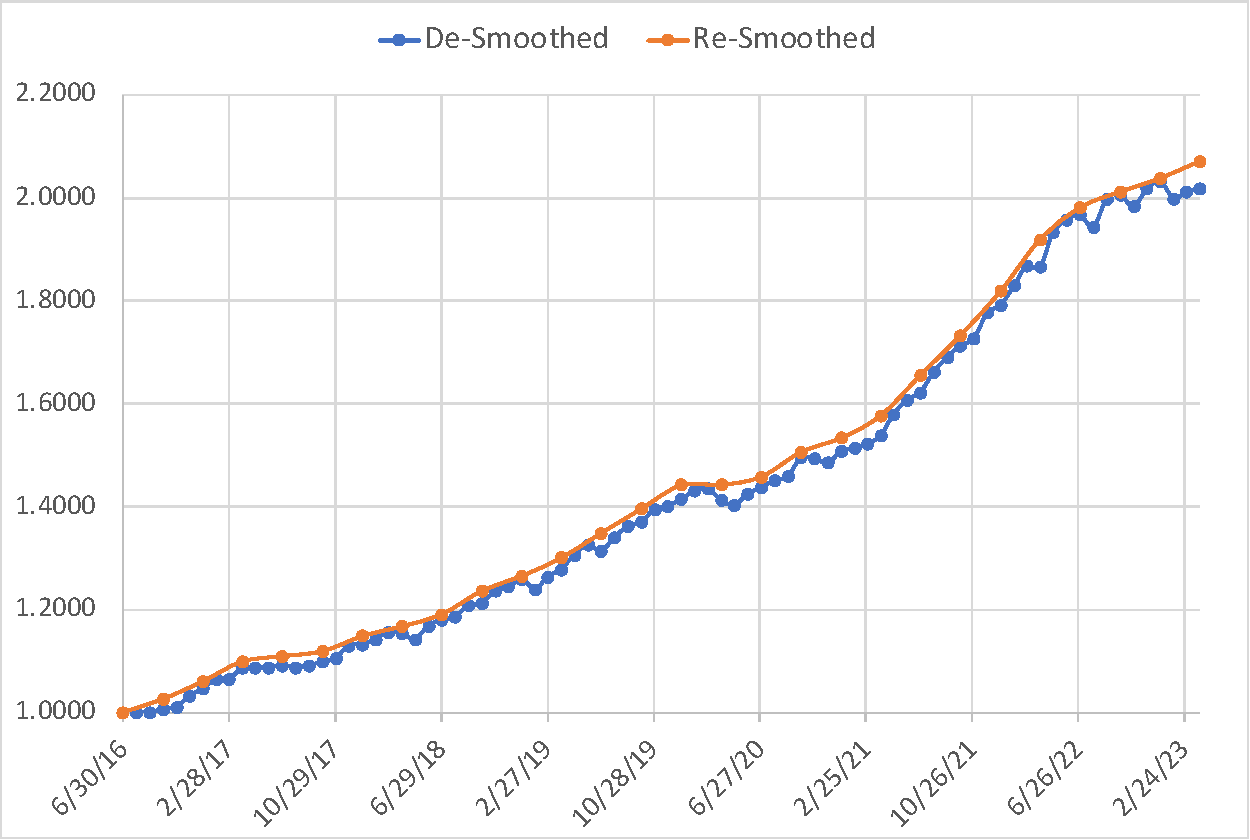
\includegraphics[width=400pt]{smoothed.pdf}
	\parbox{400pt}{\caption{An example of a fund’s de-smoothed ($x$), and re-smoothed ($y$) returns as generated by GMAM 3. The reported re-smoothed returns are quarterly, and the de-smoothed returns are monthly. Shown here is the cumulative return of \$1 invested in each of the set of returns. }}
\end{figure}


It is well-known in the finance practitioner literature that returns from alternative investment such as PE, hedge funds, or real estate funds, are highly serially correlated (see, for example, \cite{getmansky_etal}). In other words, past values are correlated with present values. The serial correlation mentioned here occurs because of the lack of liquidity in the fund itself or some of the assets held within it. For instance, these illiquid assets could be ones that don't trade frequently, making it challenging to always determine their market prices. When funds contain such illiquid assets, their reported returns may seem steadier than their actual economic returns (returns that consider all available market information about those securities). This can lead to a downward bias in estimating return variance and result in positive serial return correlation. \\

It is also well-known that returns from real estate funds, are lagged (\cite{geltner1993}). For instance, for many funds, returns are compiled and reported quarterly. But valuations of many properties included in the funds are effectively updated only annually. Each quarter some properties have their valuations updated, and others do not. Those properties that don't get a new valuation within a quarter carry over their last known value into the current quarter. \\

Finally, Financial Accounting Standard 157, released by the FASB in 2006 during the run-up to the financial crisis of that time, and now called Accounting Standards Code Topic 820, required companies to mark their assets to market. This was a radical change from historic cost accounting and required LPs to periodically mark the assets to market, even though markets in many portfolio companies are illiquid. This backwards appraisal may also result in a managerial bias towards smoothing asset values. \\

The latent returns $x_{i,t}$, henceforth just $x$ for notational simplicity, generated above are not smoothed. They are the true economic returns. Since GMAM 3 attempts to mimic true reported returns, we must re-smooth the latent returns to reflect the reported returns so that investors can appropriately compare their investments in PE with publicly available investments. In GMAM 3, this is done using a moving average (MA) process with smoothing parameters estimated using a Bayesian linear regression. Note that the MA is defined in an econometric sense, and not in a literal sense, although it may be interpreted as such. More specifically, the final returns presented to the user are re-smoothed using the following process:
\begin{equation}
\label{eq:y}
	y=\Phi x
\end{equation}

where $y$ are the reported returns and $\Phi$ is a matrix consisting of smoothing coefficients, $\phi$ and $\tilde{\phi}$. More specifically, when both $x$ and $y$ have the same reporting frequency,
\begin{equation}
\label{eq:phi}
	\Phi =
	\begin{bmatrix}
		\phi_{1} & \cdots & \phi_{P} & \tilde{\phi}_{P+1} & 0 & 0 & 0 & 0 & 0\\
		0 & \phi_{1} & \cdots & \phi_{P} & \tilde{\phi}_{P+1} & \cdots & \cdots & \cdots & 0\\
		\vdots & \ddots & \ddots & \ddots & \ddots & \ddots & \ddots & \ddots & \vdots\\
		0 & \cdots & \cdots & \cdots & \phi_{1} & \cdots & \phi_{P} & \tilde{\phi}_{P+1} & 0\\
		0 & \cdots & \cdots & \cdots & \cdots & \phi_{1} & \cdots & \phi_{P} & \tilde{\phi}_{P+1}
	\end{bmatrix} 
\end{equation}

$\phi$ is a vector of $P$ unrestricted coefficients, and $\tilde{\phi}$ is a vector of $P + \Delta t$ restricted and unrestricted coefficients. $P$ and $\Delta t$ represent terms that map the observation period of the reported, smoothed returns $y$ to the latent, de-smoothed returns, $x$. In particular,
\begin{align}
	y_{s} 	&= \left(\tilde{\phi}_{1:\left(P+\Delta t\right)}\right)'x_{(t[s]-P-\Delta t+1):t[s]}+\varepsilon_{t}^{y}	\\
			&= \left(\tilde{\phi}_{\left(P+1\right):\left(P+\Delta t\right)}\right)'x_{\left(t[s]-\Delta t+1\right):t[s]}+\phi'x_{(t[s]-P):\left(t[s]-\Delta t\right)}+\varepsilon_{t}^{y}
\end{align}

The reported returns are $y_s$ s.t. $s \in 1:S$, and the latent returns are $x_t$ s.t. $t \in 1:T$. In equation \eqref{eq:phi} above, $S = T$, and the reported returns and de-smoothed returns have the same frequency. However, $S$ may not always equal $T$, such as when the reported returns are quarterly, and the de-smoothed returns are monthly\footnote{Our factor returns are almost always monthly, as are the de-smoothed returns.}. To resolve this, the following formula maps $t$ to $s$:
\begin{equation}
	t(s) = P + (s \times \Delta t)
\end{equation}

For example, if the reported returns $y$ are quarterly, and the latent returns $x$ are monthly, $P=3$, and $\Delta t = 3$ (since each quarter consists of three months). And so, for the first quarter, $s = 1$, and $t = 6$. When $\Delta t > 1$, the $\tilde{\phi}_j$, for $j \in 1:\Delta t$ must add up to the same value, $\forall j$. If not, months that fall earlier in the quarter will have a different long-run impact on NAV than months later in the quarter. In the current version of GMAM 3 in production, they add up to 3 when reported returns are quarterly, and they add up to 1 when reported returns are monthly\footnote{Note that the vector $\phi \in \tilde{\phi}$. For quarterly reported data, say $\phi = [a, b, c]^\prime$ where $a, b, c \in \mathbb{R}$. Then, $\tilde{\phi} = [a, b, c, 1-a, 1-b, 1-c]^\prime$ and the sum of all terms in $\tilde{\phi}$ is 3. For monthly reported data, say $\phi = [a, b, c, d, e]^\prime$ where $a, b, c, d,e \in \mathbb{R}$. Then $\tilde{\phi} = [a, b, c, d, e, 1-a-b-c-d-e]^\prime$ and the sum of all terms in $\tilde{\phi}$ here, is 1. This process is also described in more detail in the Appendix.}.  \\

The economic assumption behind this process is that the observed fund returns $y$ are a weighted average of the fund’s economic returns $x$ over the most recent ($P + \Delta t$) periods, including the current period. The econometric implications of this are that under the given assumption, the observed fund returns follow a MA process of order $P + \Delta t$. \\

This restriction is similar to \cite{getmansky_etal} where the observed return ($R_t^0$) for some period $t$, is a weighted average of the 	``true'' returns ($R_t^C$) over the most recent $k+1$ periods: $R_t^0 = \theta_0 R_t^C + \cdots + \theta_k R_(t-k)^C$, with $\sum_{i=0}^k \theta_i  = 1$ to ensure that all information is eventually incorporated into observed returns, and $\theta_i \in [0,1]$ for $i = 1, \ldots, k$. In our case the observed returns are the reported returns, $y$, the ``true'' returns are the latent returns generated using the factors, $x$, and the $\theta_i$ terms from \cite{getmansky_etal} are denoted as $\phi_i$ in our estimation process. They are generated using a multivariate normal distribution in the hierarchical Bayesian model, as follows:

\begin{equation}
\label{eq:phi_dist}
	p\left(\phi|rest\right) \sim MN\left(\phi_{0},\frac{1}{\tau_{y}\tau_{\phi}}M_{0}^{-1}\right)
\end{equation}

where $\tau_y$ is a global precision parameter estimated for independent measurement using a Gamma-distributed prior: $p( \tau_y ) \sim Gamma \left( \alpha_{y_0}, \zeta_{y_0} \right)$ with given shape hyperparameter,$\alpha_{y_0}$, and given inverse scale hyperparameter, $\zeta_{y_0}$;  $\tau_\phi$ is a global precision multiplier parameter, distributed as $p( \tau_\phi ) \sim Gamma \left(\alpha_{\phi_0}, \zeta_{\phi_0} \right)$ with given shape and inverse scale hyperparameters; $M_0$ is a $P \times P$ matrix consisting of precision hyperparameters for $\phi_0$; and $\phi_0$ is a hyperparameter (i.e., fed into the model). \\

And the complete posterior distribution of $y$ is given by:
\begin{equation}
\label{eq:y_dist}
	p \left( y \mid rest \right) \sim MN \left( \Phi x,\frac{1}{\tau_{y}}I\right))
\end{equation}

with $\Phi$, $x$, and $\tau_y$ defined as above; and $I$ is an identity matrix used for computational purposes.

\subsection{A Brief Digression on Priors}
Since we are beginning to describe our posterior distributions with their respective priors, it might make sense to motivate some understanding about prior distributions in the context of a hierarchical Bayesian model. \\

Priors, while influencing the results with fewer datapoints and noisier data, do not ultimately matter much as data increases. Priors are, of course, essential in Bayesian analysis. However, their influence generally decreases as the amount of data increases, especially if the data is strongly informative. In theory, Bayesian models exhibit a property known as `consistency.' This means that as the sample size grows to infinity, the posterior distribution of the parameter of interest will converge to the ``true'' parameter value\footnote{In the frequentist sense of the word.}, assuming the model is correctly specified. In such a scenario, the choice of prior becomes less critical as the sample size increases. \\

That said, the use of the gamma distribution with an inverse scale parametrization above is convenient for several reasons:
\begin{enumerate}
	\item Conjugacy: conjugate priors are advantageous for computational and analytical simplicity. 
	\item Positive Values: the gamma distribution is defined for positive values only.
	\item Informative and Non-Informative Settings: the gamma distribution can be used to encode both informative and non-informative priors. By adjusting its parameters, you can represent strong prior beliefs or specify a prior that has minimal influence on the posterior, allowing the data to drive the inference.
	\item Regularization and Stability: In Bayesian hierarchical models, the use of gamma priors can help in regularizing the estimates, particularly in complex models or in the presence of limited data. This can prevent overfitting and improve the model's stability and predictive performance.
\end{enumerate}

%The variables modeled as beta and Bernoulli distributions are used in the SSVS regression outlined earlier. In particular, γ_k, has only two values so modeling it as Bernoulli makes sense in this context.

\subsection{Stochastic Search Variable Selection (SSVS)}
\label{subsec:spike_and_slab}

\begin{figure}[!h]
	\centering
	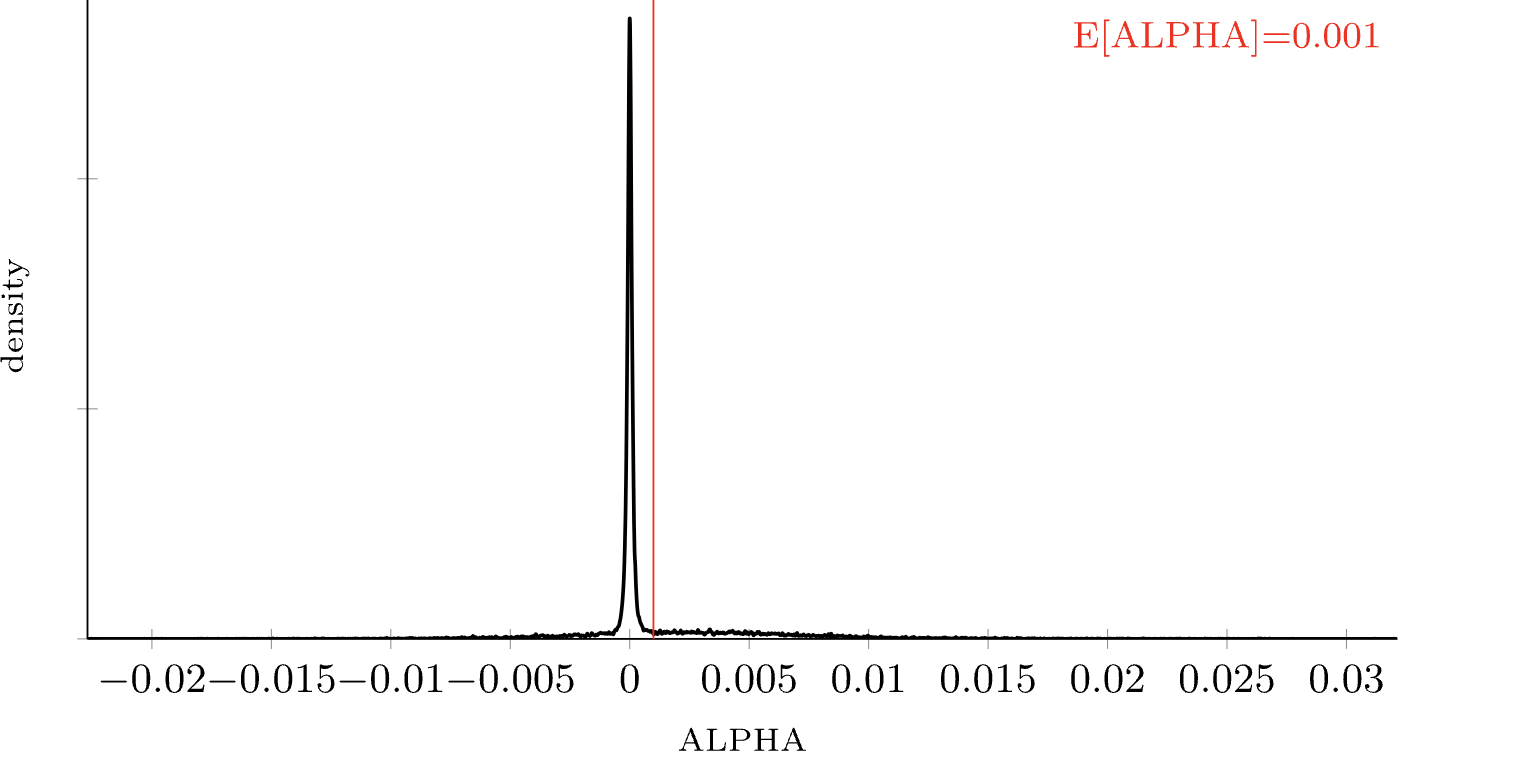
\includegraphics[width=400pt]{clinton_alpha_1_ares.png}
	\parbox{400pt}{\caption{The probability mass function of a fund's intercept term ($\beta_0$) from the SSVS (spike and slab) regression. We see a spike here because for this particular fund the probability mass is concentrated around zero with a small positive tilt. Additionally, there is low evidence of an intercept term. We have 14 months of history for this fund. }}
\end{figure}

As mentioned above, the regression performed to estimate $x$ is using a SSVS technique which defines prior regression coefficient variances consistent with inclusion or effective exclusion. In other words, it is a predictor selection technique. Such techniques commonly focus on which predictors to retain, though they also aim for improved predictive performance through developing an encompassing model, or model simplification without adversely affecting predictive accuracy (\cite{piironen_vehtari}).  Formal model choice is simplified for normal linear regression, as marginal likelihoods may be obtained analytically, but for many predictors, comparison of the many possible models becomes infeasible. \\

An imperfect analogy is stepwise regression using AIC or BIC as a selection criterion. However, when the number of regressors is large (as mentioned above, we have 13), the computational requirements for these procedures can be prohibitive. A common workaround is to use a heuristic method to restrict attention to a potential subset of regressors, i.e., include or exclude variables, based on $R^2$ considerations (say). \\

SSVS uses a Bayesian approach with a normal mixture model for regression analysis. In this method, selector variables are employed to pinpoint which subsets of predictors are worth considering. It works by identifying those predictors that have a higher chance of being relevant, based on their posterior probability. To do this, SSVS uses a technique called Gibbs sampling\footnote{Gibbs sampling is a statistical technique used for generating sequences of samples from the probability distribution of multiple variables. It's a kind of Markov Chain Monte Carlo (MCMC) method. It is particularly useful in scenarios where directly sampling from the joint distribution is difficult, but sampling from the conditional distribution of each variable is feasible.}. This approach helps to sample from the distribution of all possible subsets of predictors. The subsets that show up more often in these samples are considered promising because they have a higher probability of being relevant. \\

We use the SSVS technique of \cite{george_and_mcculloch}, also known as a \textbf{spike and slab regression}. The term was coined by \cite{mitchell_beauchamp} and referred to the prior for the regression coefficients used in their Bayesian hierarchy. This prior was chosen such that the regression parameters were mutually independent with a two-point mixture distribution made up of a uniform flat distribution (the slab) and a degenerate distribution at zero (the spike). \\

\cite{ishwaran2005spike} characterize a spike and slab model as being any model with a Bayesian hierarchy specified as follows:
\begin{align*}
	p(y \mid X, \beta, \sigma^2) &\sim N( X\beta, \sigma^2 I_n)	\\
	p(\beta \mid \gamma) &\sim N (0, \Gamma) \\
	\gamma \coloneqq (\gamma_1, \ldots, \gamma_p)^T &\sim \pi (\cdot) \\
	p(\sigma^2) &\sim \mu( \cdot )
\end{align*}

Here, $\beta = (\beta_1, \ldots, \beta_p)^T$ is the regression vector, and $\Gamma = diag(\gamma_k)_{1 \leq k \leq p}$ is its $p \times p$ hypervariance matrix. The prior $\pi$ for the hypervariance $\gamma$ plays a critical role in how effective the technique is for variable selection. A successful and popular choice of $\pi$ are priors that make use of mixture distributions involving a spike near zero. In \cite{george_and_mcculloch}, the prior for $\gamma_k$ was assumed to have a two-component distribution of the form:
\begin{equation*}
	p \left( \gamma_k \mid \tau_k, c_k, \overline{\omega}_k \right) \myeq (1 - \overline{\omega}_k \delta_{\tau_k} (\cdot) + \overline{\omega}_k \delta_{c_k \tau_k} (\cdot), \quad k = 1, \ldots p.
\end{equation*}

 The value for $\tau_k > 0$ (the spike) is chosen to be some small value, where ``small'' is typically based on the data at hand, while $c_k > 0$, also data-specific, is chosen so that $c_k \tau_k$ (the slab) is sufficiently large. Selecting the two hyperparameters in this way allows $\gamma_k$ to be small or large, and this in turn enables the posterior of $\beta_k$ to shrink towards zero or be some nonzero value. The values $(\overline{\omega}_k)_{k=1}^p$ are complexity parameters that influence the likelihood of a coefficient being shrunk towards zero. In principle, each variable can have a unique complexity value, but a common practice is to set $\overline{\omega}_k = 1/2, \forall k$, in which case the prior will be referred to as an indifference prior. \\

\begin{figure}[!h]
	\centering
	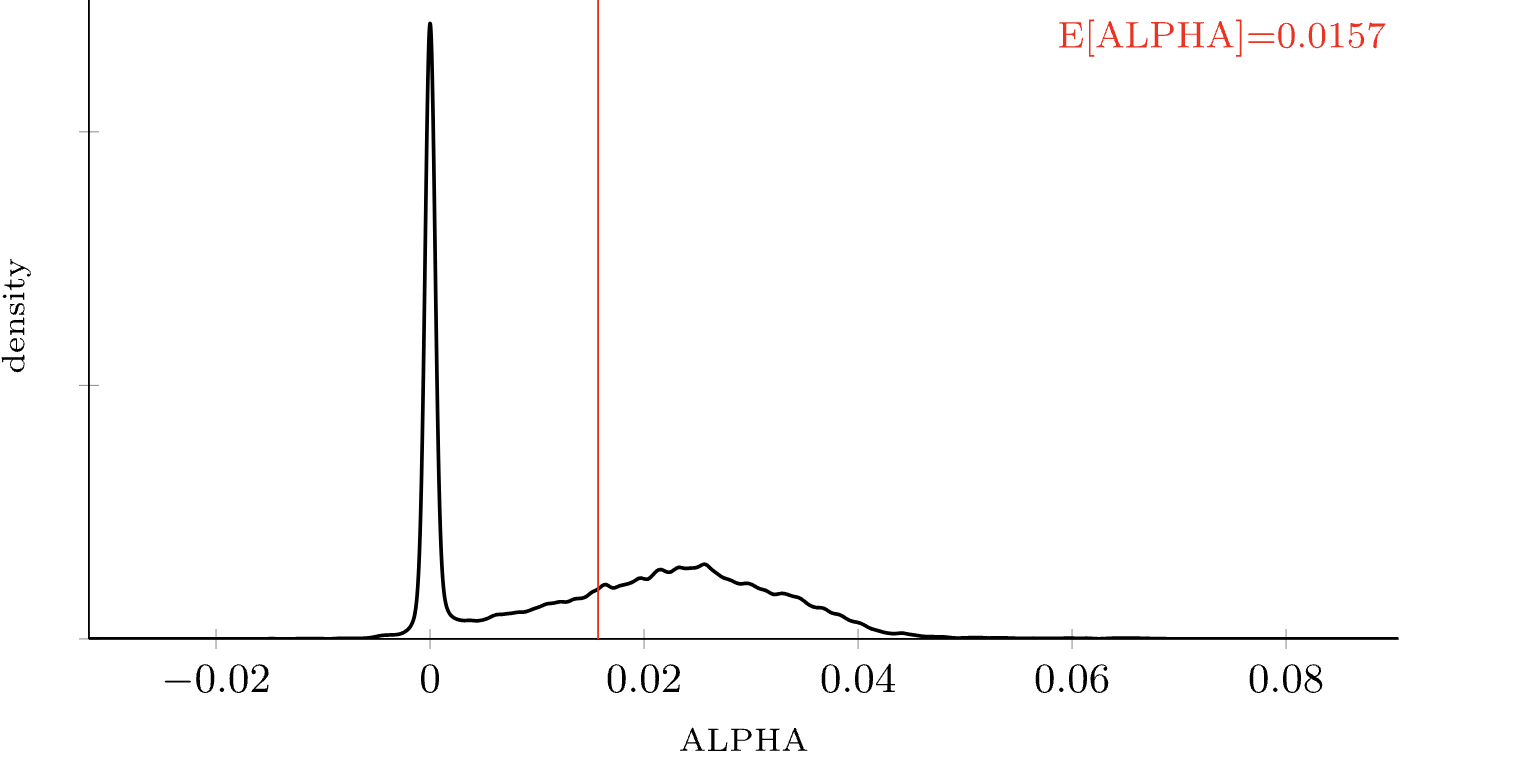
\includegraphics[width=400pt]{clinton_alpha_2_hl_sfvi.png}
	\parbox{400pt}{\caption{The probability mass function of a fund's intercept term ($\beta_0$) from the SSVS (spike and slab) regression. Though we see a spike here, the bulk is in the long right tail representing substantial upside and a significantly greater weight of evidence for a positive alpha. This fund has over two years of history.}}
\end{figure}

For our model, we use a Bernoulli or binomial prior on $\gamma_k$, the selector variable:
\begin{equation}
\label{eq:gamma_k_dist}
	p\left(\gamma_{k}\right) \sim Bern\left(\omega\right)
\end{equation}

Here, $p \left( \omega \right) \sim Beta \left(\kappa_{0},\delta_{0}\right)$ which is the probability of factor selection with hyperparameters $\kappa_0$ and $\delta_0$ specified as given. $\gamma_k$ for $k \in 1:K$ is a $K \times 1$ vector and selector variable used to determine which of the thirteen factors are economically significant in a probabilistic sense. Initially, each of the factors have an equally likely chance of being included. Conditional on a factor being in the regression, we specify a prior distribution for the regression coefficient associated with that variable. In our case, this is multivariate normal:
\begin{align}
	p\left(\beta|rest\right) &\sim MN\left(\beta_{0}+D^{-1}\beta_{0}^{\Delta},\frac{1}{\tau_{x}\tau_{y}\tau_{\beta}}\left[DA_{0}D\right]^{-1}\right)	\label{eq:beta_dist}\\
	d_{k} &= \sqrt{\gamma_{k}+(1-\gamma_{k})\frac{1}{v^{2}})} \label{eq:d_k}
\end{align}

Here, $\beta_0$ is the prior mean of $\beta$ conditional on exclusion (i.e., when $\gamma_k = 0$); $\beta_0^\Delta$ is the shift in the prior mean of $\beta$ conditional on inclusion (i.e., when $\gamma_k = 1$); $d_k$ for $k \in 1:K$ is a $K \times 1$ vector -- a function of $\gamma$ which adjusts $\beta$ for sparsity; $D$ is a $K \times K$ matrix with $D = diag(d_k)$; and $\nu$ is the variance of the spike distribution as a fraction of the slab variance. And finally, $\tau_x$, $\tau_y$, and $\tau_\beta$ are all gamma-distributed with shape and inverse-scale hyperparameters as shown earlier. \\

\begin{figure}[!h]
	\centering
	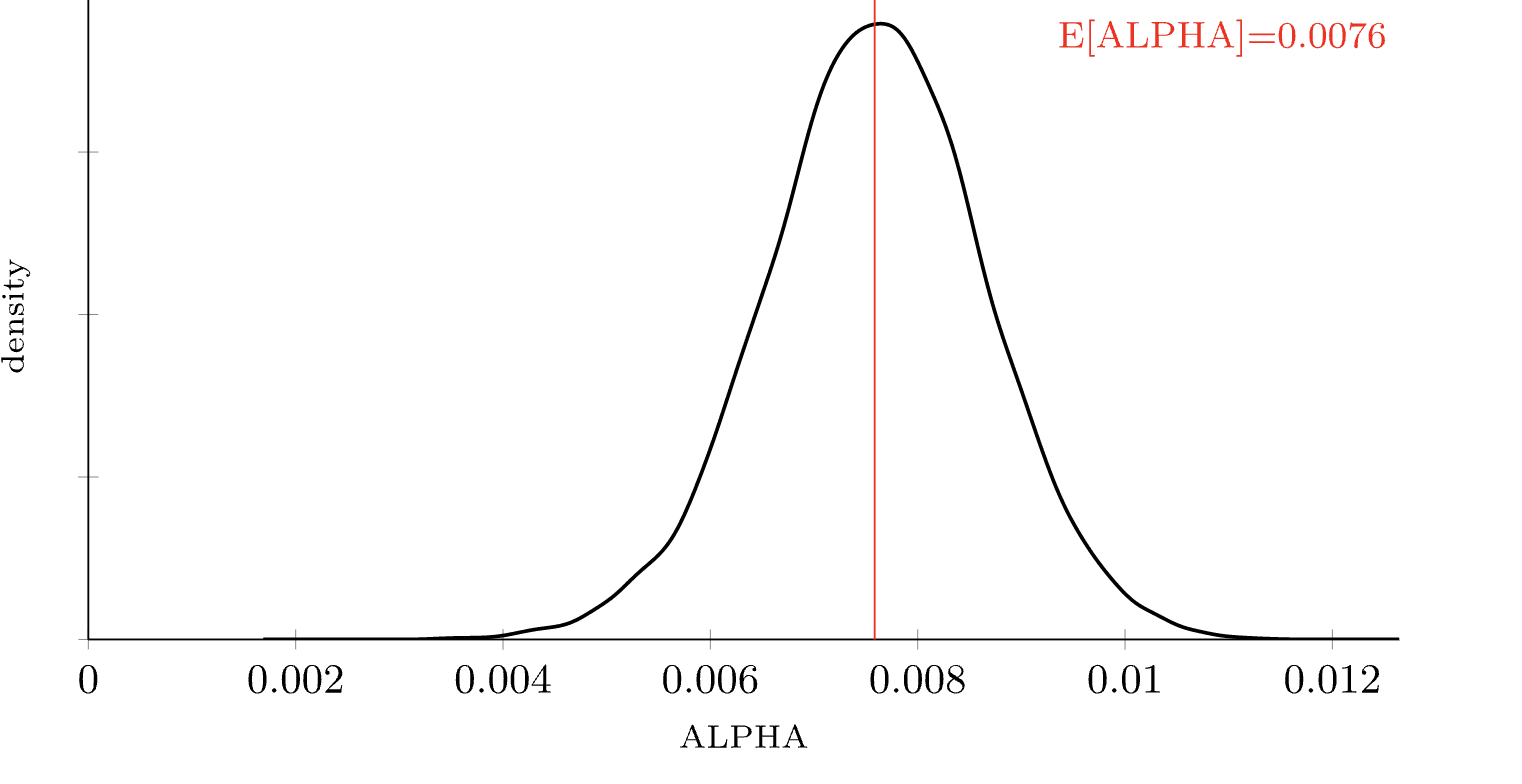
\includegraphics[width=400pt]{clinton_alpha_3_preqin.png}
	\parbox{400pt}{\caption{The probability mass function of a fund index intercept term ($\beta_0$) from the SSVS (spike and slab) regression. This index has almost twenty years of history and clearly shows positive alpha, though its magnitude is still uncertain.}}
\end{figure}

\section{Conclusion}
We use a hierarchical Bayesian model to generate fund returns when data is sparse and noisy. The data generation process includes de-smoothed returns, generated using a spike and slab regression, and re-smoothed returns used to mimic reported returns. Our technique provides a systematic and rigorous way by which fund performance can be quantified.

\newpage

\singlespacing
\setlength\bibsep{3pt}

\bibliographystyle{plainnat}
\setcitestyle{numbers}
\bibliography{tech_manual}

%\newpage
%
%\section{Appendix}
%The complete generative process is given by:
%\begin{align}
%	p\left(y|rest\right)	&\sim	MN\left(X_{L}R\phi+x_{S},\frac{1}{\tau_{y}}I\right) \quad \text{equivalently,~}MN\left(\Phi x,\frac{1}{\tau_{y}}I\right) \tag{\ref{eq:y_dist}}\\
%	p\left(x|rest\right)	&\sim	MN\left(F\beta+r,\frac{1}{\tau_{x}\tau_{y}}\Psi^{-1}\right)\\
%	p\left(\phi|rest\right)	&\sim	MN\left(\phi_{0},\frac{1}{\tau_{y}\tau_{\phi}}M_{0}^{-1}\right) \tag{\ref{eq:phi_dist}}\\
%	p\left(\beta|rest\right)	&\sim	MN\left(\beta_{0}+D^{-1}\beta_{0}^{\Delta},\frac{1}{\tau_{x}\tau_{y}\tau_{\beta}}\left[DA_{0}D\right]^{-1}\right) \tag{\ref{eq:beta_dist}}\\
%	d_{k}\			&=		(\gamma_{k}+(1-\gamma_{k})\frac{1}{v^{2}})^{0.5} \tag{\ref{eq:d_k}}\\
%	p\left(\gamma_{k}\right)&\sim	Bern\left(\omega\right) \tag{\ref{eq:gamma_k_dist}}\\
%	p\left(\omega\right)	&\sim 	Beta\left(\kappa_{0},\delta_{0}\right)\\
%	p\left(\tau_{y}\right)	&\sim	Gamma\left(\alpha_{y0},\zeta_{y0}\right)\\
%	p\left(\tau_{x}\right)	&\sim	Gamma\left(\alpha_{x0},\zeta_{x0}\right)\\
%	p\left(\psi_{t}\right)	&\sim	Gamma\left(\nu/2,\nu/2\right)\\
%	p\left(\nu\right)		&\sim	Gamma\left(\alpha_{\nu0},\zeta_{\nu0}\right)\\
%	p\left(\tau_{\phi}\right)&\sim	Gamma\left(\alpha_{\phi0},\zeta_{\phi0}\right)\\
%	p\left(\tau_{\beta}\right)&\sim	Gamma\left(\alpha_{\beta0},\zeta_{\beta0}\right)
%\end{align}
%
%Note that here $y$ can be written in two forms using matrix notation. When $x$ and $y$ have the same frequency:
%\begin{equation}
%	y = \Phi x 			= X_{L}R\phi+x_{S}		\tag{\ref{eq:y}}
%\end{equation}
%
%Where
%\begin{equation}
%\label{eq:y_matrix}
%	X_{L}R\phi+x_{S}	= 	\begin{bmatrix}
%							x_{1} & x_{2} & \cdots & x_{P-1} & x_{P} & x_{P+1}\\
%							x_{2} & x_{3} & \cdots & x_{P} & x_{P+1} & x_{P+2}\\
%							\vdots & \vdots & \ddots & \vdots & \vdots & \vdots\\
%							x_{T-P-1} & x_{T-P} & \cdots & x_{T-3} & x_{T-2} & x_{T-1}\\
%							x_{T-P} & x_{T-P+1} & \cdots & x_{T-2} & x_{T-1} & x_{T}
%						\end{bmatrix} 
%						\left[R \right]
%						\begin{bmatrix}
%							\phi_{1}\\
%							\phi_{2}\\
%							\vdots\\
%							\phi_{P-1}\\
%							\phi_{P}
%						\end{bmatrix} +
%						\begin{bmatrix}
%							x_{P+1}\\
%							x_{P+2}\\
%							\vdots\\
%							x_{T-1}\\
%							x_{T}
%						\end{bmatrix}
%\end{equation}
%And
%\begin{equation*}
%	R = \begin{bmatrix}
%			1 & 0 & \cdots & 0 & 0\\
%			0 & 1 & \cdots & 0 & 0\\
%			\vdots & \vdots & \ddots & \vdots & \vdots\\
%			0 & 0 & \cdots & 1 & 0\\
%			0 & 0 & \cdots & 0 & 1\\
%			-1 & -1 & \cdots & -1 & -1
%		\end{bmatrix}
%\end{equation*}
%
%To generalize to other frequencies, recall that $t\left[s\right]\equiv P+s*\Delta t$ and define:
%\begin{align}
%\begin{split}
%	\Phi_{sj}	\equiv	&\begin{cases}
%						\phi_{P-\left(t\left[s\right]-\Delta t-j\right)} & 1\le P-(t\left[s\right]-\Delta t-j)\le P\\
%						1-\left(\iota_{\Delta t-\left(t\left[s\right]-j\right)}^{\phi}\right)'\phi & t\left[s\right]-\Delta t<j\le t\left[s\right]\\
%						0 & \text{otherwise}	
%					\end{cases} \\
%	X_{Lsj}	\equiv	&x_{t\left[s\right]-\left(P+\Delta t-j\right)}	\\	
%	\iota_{pl}^{\phi}
%			\equiv	&\begin{cases}
%						1 & p+l\mod\Delta t=0\\
%						0 & \text{otherwise}
%					\end{cases} 
%\end{split}
%\end{align}
%
%The above matrix formulation \eqref{eq:y_matrix} can be generalized by only including rows of $X_{L}$ where $t\in\left\{ t\left[1...S\right]\right\}$ and adjusting the restriction matrix. The general version is then:
%\begin{equation}
%	y=\Phi x =	X_{L}R\phi+x_{S}, \quad \text{s.t.~} x_{S} =	X_{L}\iota_{\Delta t} \tag{\ref{eq:y}}
%\end{equation}
%where $\iota_{\Delta t}$ is a vector of $P$ zeros followed by $\Delta t$ ones, making $x_{S}$ the sum of the last $\Delta t$ columns of $X_{L}$.
%
%\subsection{Complete Posterior Distribution}
%The complete posterior distribution is given by:
%\begin{align}
%\begin{split}
%	p\left(\Theta|y,F\right) 	&\propto p\left(y|x,\gamma,\omega,\beta,\phi,\tau_{x},\tau_{y},\tau_{\phi},\tau_{\beta},\psi,\nu,F\right)\times p\left(x|\beta,\phi,\tau_{x},\tau_{y},\psi,F\right)\\
%						&\times p\left(\phi|\tau_{y},\tau_{\phi}\right)\times p\left(\beta|\gamma,\tau_{x},\tau_{y},\tau_{\beta}\right)\times p\left(\gamma|\omega\right)\times p\left(\omega\right)\\
%						&\times p\left(\psi|\nu\right)\times p\left(\nu\right)\times p\left(\tau_{x}\right)\times p\left(\tau_{y}\right)\times p\left(\tau_{\phi}\right)\times p\left(\tau_{\beta}\right)\\
%						&=MN\left(y;\Phi x,\frac{1}{\tau_{y}}I\right)\times MN\left(x;F\beta+r,\frac{1}{\tau_{x}}\Psi^{-1}\right)\\
%						&\times MN\left(\phi;\phi_{0},\frac{1}{\tau_{y}\tau_{\phi}}M_{0}^{-1}\right)\times MN\left(\beta;\beta_{0}+D^{-1}\beta_{0}^{\Delta},\frac{1}{\tau_{x}\tau_{\beta}}\left[DA_{0}D\right]^{-1}\right)\\
%						&\times\prod_{k=1}^{K}Bern\left(\gamma_{k};\omega\right)\times Beta\left(\omega;\kappa_{0},\delta_{0}\right)\\
%						&\times\prod_{t=1}^{T}Gamma\left(\psi;\nu/2,\nu/2\right)\times Gamma\left(\nu;\alpha_{\nu0},\zeta_{\nu0}\right)\\
%						&\times Gamma\left(\tau_{x};\alpha_{x0},\zeta_{x0}\right)\times Gamma\left(\tau_{y};\alpha_{y0},\zeta_{y0}\right)\\
%						&\times Gamma\left(\tau_{\phi};\alpha_{\phi0};\zeta_{\phi0}\right)\times Gamma\left(\tau_{\beta};\alpha_{\beta0},\zeta_{\beta0}\right)
%\end{split}
%\end{align}
%
%\subsection{Posterior of $\phi$}
%\begin{equation}
%	\log p\left(\phi|rest\right) = \log MN\left(\phi;\mu_{\phi},\Lambda_{\phi}^{-1}\right)+c_{4}^{\phi}
%\end{equation}
%where
%\begin{align*}
%\begin{split}
%	\Lambda_{\phi}	&=	\tau_{y}\left(\tilde{X}_{L}'\tilde{X}_{L}+\tau_{\phi}M_{0}\right)\\
%	\mu_{\phi} 	&=	\tau_{y}\Lambda_{\phi}^{-1}\left(\tilde{X}_{L}'\tilde{y}+\tau_{\phi}M_{0}'\phi_{0}\right)\\
%	c_{1}^{\phi}	&=	\frac{S+P}{2}\log\left(\frac{\tau_{y}}{2\pi}\right)+\frac{P}{2}\log\tau_{\phi}+\frac{1}{2}\log det\left(M_{0}\right)\\
%				&+\log\Bigg[MN\left(x;F\beta+r,\frac{T}{\tau_{x}\tau_{y}}\Psi^{-1}\right)\times MN\left(\beta;\beta_{0}+D^{-1}\beta_{0}^{\Delta},\frac{1}{\tau_{x}\tau_{y}\tau_{\beta}}\left[DA_{0}D\right]^{-1}\right)\\
%				&\times\prod_{k=1}^{K}Bern\left(\gamma_{k};\omega\right)\times Beta\left(\omega;\kappa_{0},\delta_{0}\right)\times\prod_{t=1}^{T}Gamma\left(\psi;\nu/2,\nu/2\right)\\
%				&\times Gamma\left(\nu;\alpha_{\nu0},\zeta_{\nu0}\right)\times Gamma\left(\tau_{x};\alpha_{x0},\zeta_{x0}\right)\times Gamma\left(\tau_{y};\alpha_{y0},\zeta_{y0}\right)\\
%				&\times Gamma\left(\tau_{\beta};\alpha_{\beta0},\zeta_{\beta0}\right)\times Gamma\left(\tau_{\phi};\alpha_{\phi0},\zeta_{\phi0}\right)\Bigg]+c^{ev}\\
%	c_{2}^{\phi}	&=	c_{1}^{\phi}-\frac{\tau_{y}}{2}\left[\tau_{\phi}\phi_{0}'M_{0}\phi+\tilde{y}'\tilde{y}\right]\\
%	c_{3}^{\phi}	&= 	c_{2}^{\phi}+\frac{1}{2}\mu_{\phi}'\Lambda_{\phi}\mu_{\phi}\\
%	c_{4}^{\phi}	&=	c_{3}^{\phi}+\frac{P}{2}\log2\pi-\frac{1}{2}\log det\Lambda_{\phi}\\
%	c_{ev}		&=	-\log p\left(y_{t}\right)
%\end{split}
%\end{align*}
%The last constant makes the full posterior into a valid probability distribution. \\
%
%Note that it may make sense to impose additional restrictions not easily captured by $R$. For instance, the prior distribution can be truncated to force $\phi\in\left[0,1\right]$. With this restriction, the above analysis applies over the interval, with the support of the posterior and prior distribution truncated and re-normalized as appropriate. Then the approximate posterior of $\phi$ is:
%
%\begin{equation}
%	\log q\left(\phi\right) = \log MN\left(\phi;\overline{\mu}_{\phi},\overline{\Lambda}_{\phi}^{-1}\right)+\overline{c}_{4}^{\phi}
%\end{equation}
%
%where
%\begin{align*}
%\begin{split}
%	\overline{\Lambda}_{\phi}	&=	E[\tau_{y}]\left(E\left[\tilde{X}_{L}'\tilde{X}_{L}\right]+E\left[\tau_{\phi}\right]E\left[M_{0}\right]\right)\\
%	\overline{\mu}_{\phi}		&=	E[\tau_{y}]\Lambda_{\phi}^{-1}\left(E\left[\tilde{X}_{L}'\tilde{y}\right]+E\left[\tau_{\phi}\right]E\left[M_{0}\right]\phi_{0}\right)\\
%	\overline{c}_{1}^{\phi}	&=	\frac{S+P}{2}E\left[\log\left(\frac{\tau_{y}}{2\pi}\right)\right]+0.5\log det\left(M_{0}\right)+\frac{P}{2}\log\tau_{\phi}\\
%						&+E_{-\phi}\log\Bigg[MN\left(x;F\beta+r,\frac{1}{\tau_{x}\tau_{y}}\Psi^{-1}\right)\times MN\left(\beta;\beta_{0}+D^{-1}\beta_{0}^{\Delta},\frac{1}{\tau_{x}\tau_{y}\tau_{\beta}}\left[DA_{0}D\right]^{-1}\right)\\
%						&\times\prod_{k=1}^{K}Bern\left(\gamma_{k};\omega\right)\times Beta\left(\omega;\kappa_{0},\delta_{0}\right)\times\prod_{t=1}^{T}Gamma\left(\psi;\nu/2,\nu/2\right)\\
%						&\times Gamma\left(\nu;\alpha_{\nu0},\zeta_{\nu0}\right)\times Gamma\left(\tau_{x};\alpha_{x0},\zeta_{x0}\right)\times Gamma\left(\tau_{y};\alpha_{y0},\zeta_{y0}\right)\\
%						&\times Gamma\left(\tau_{\beta};\alpha_{\beta0},\zeta_{\beta0}\right)\times Gamma\left(\tau_{\phi};\alpha_{\phi0},\zeta_{\phi0}\right)\Bigg]+c^{ev}\\
%	\overline{c}_{2}^{\phi}	&= 	\overline{c}_{1}^{\phi}-\frac{E[\tau_{y}]}{2}\left(E\left[\tilde{y}'\tilde{y}\right]+E\left[\tau_{\phi}\right]\phi_{0}'E\left[M_{0}\right]\phi_{0}\right)\\
%	\overline{c}_{3}^{\phi}	&=	\overline{c}_{2}^{\phi}+\frac{1}{2}\left(\overline{\mu}_{\phi}'\overline{\Lambda}_{\phi}\overline{\mu}_{\phi}\right)\\
%	\overline{c}_{4}^{\phi}	&=	\overline{c}_{3}^{\phi}+\frac{P}{2}\log2\pi-\frac{1}{2}\log\left(det\left(\overline{\Lambda}_{\phi}\right)\right)
%\end{split}
%\end{align*}
%
%\subsection{Posterior of $x$}
%\begin{equation}
%	\log p\left(x|rest\right) = \log MN\left(x;\mu_{x},\Lambda_{x}^{-1}\right)+c_{4}^{x}
%\end{equation}
%where
%\begin{align*}
%\begin{split}
%	\Lambda_{x} 	&=	\tau_{y}\left(\Phi'\Phi+\tau_{x}\Psi\right)\\
%	\mu_{x}		&=	\tau_{y}\Lambda_{x}^{-1}\left(\Phi'y+\tau_{x}\Psi\left(r+F\beta\right)\right)\\
%	c_{1}^{x}		&=	\frac{S+T}{2}\log\left(\frac{\tau_{y}}{2\pi}\right)+\frac{T}{2}\log\tau_{x}+\frac{1}{2}\log Det\left(\Psi\right)\\
%				&+\log\Bigg[MN\left(\phi;\phi_{0},\frac{1}{\tau_{y}\tau_{\phi}}M_{0}^{-1}\right)\times MN\left(\beta;\beta_{0}+D^{-1}\beta_{0}^{\Delta},\frac{1}{\tau_{x}\tau_{y}\tau_{\beta}}\left[DA_{0}D\right]^{-1}\right)\\
%				&\times\prod_{k=1}^{K}Bern\left(\gamma_{k};\omega\right)\times Beta\left(\omega;\kappa_{0},\delta_{0}\right)\times\prod_{t=1}^{T}Gamma\left(\psi;\nu/2,\nu/2\right)\times Gamma\left(\nu;\alpha_{\nu0},\zeta_{\nu0}\right)\\
%				&\times Gamma\left(\tau_{x};\alpha_{x0},\zeta_{x0}\right)\times Gamma\left(\tau_{y};\alpha_{y0},\zeta_{y0}\right)\\
%				&\times Gamma\left(\tau_{x};\alpha_{x0},\zeta_{x0}\right)\times Gamma\left(\tau_{y};\alpha_{y0},\zeta_{y0}\right)\\
%				&\times Gamma\left(\tau_{\beta};\alpha_{\beta0},\zeta_{\beta0}\right)\times Gamma\left(\tau_{\phi};\alpha_{\phi0},\zeta_{\phi0}\right)\Bigg]+c^{ev}\\
%	c_{2}^{x}		&=	c_{1}^{x}-\frac{\tau_{y}\tau_{x}}{2}\left(r+F\beta\right)'\Psi\left(r+F\beta\right)-\frac{\tau_{y}}{2}y'y\\
%	c_{3}^{x}		&=	c_{2}^{x}+\frac{\mu_{x}'\Lambda_{x}\mu_{x}}{2}\\
%	c_{4}^{x}		&=	c_{3}^{x}+\frac{T}{2}\log2\pi-\log det\Lambda_{x}
%\end{split}
%\end{align*}
%
%The approximate posterior is:
%\begin{equation}
%	\log q\left(x\right) = \log\left(N\left(x;\overline{\mu}_{x},\overline{\Lambda}_{x}^{-1}\right)\right)+\overline{c}_{4}^{x}
%\end{equation}
%
%where
%\begin{align*}
%\begin{split}
%	\overline{\Lambda}_{x}	&=	E\left[\tau_{y}\right]\left(E\left[\Phi'\Phi\right]+E\left[\tau_{x}\right]E\left[\Psi\right]\right)\\
%	\overline{\mu}_{x}		&=	E\left[\tau_{y}\right]\Lambda_{x}^{-1}\left(E\left[\Phi\right]'y+E\left[\tau_{x}\right]E\left[\Psi\right]\left(F\overline{\mu}_{\beta}+r\right)\right)\\
%	\overline{c}_{1}^{x}		&=	E_{-x}\Bigg[\frac{S+T}{2}\log\frac{\tau_{y}}{2\pi}+\frac{T}{2}\log\tau_{x}+\frac{1}{2}\log det\Psi\\
%						&+\log\Bigg(MN\left(\phi;\phi_{0},\frac{1}{\tau_{y}\tau_{\phi}}M_{0}^{-1}\right)\times MN\left(\beta;\beta_{0}+D^{-1}\beta_{0}^{\Delta},\frac{1}{\tau_{x}\tau_{y}\tau_{\beta}}\left[DA_{0}D\right]^{-1}\right)\\
%						&\times\prod_{k=1}^{K}Bern\left(\gamma_{k};\omega\right)\times Beta\left(\omega;\kappa_{0},\delta_{0}\right)\times\prod_{t=1}^{T}Gamma\left(\psi;\nu/2,\nu/2\right)\times Gamma\left(\nu;\alpha_{\nu0},\zeta_{\nu0}\right)\\
%						&\times Gamma\left(\tau_{x};\alpha_{x0},\zeta_{x0}\right)\times Gamma\left(\tau_{y};\alpha_{y0},\zeta_{y0}\right)\\
%						&\times Gamma\left(\tau_{\beta};\alpha_{\beta0},\zeta_{\beta0}\right)\times Gamma\left(\tau_{\phi};\alpha_{\phi0},\zeta_{\phi0}\right)\Bigg)\Bigg]+c^{ev}\\
%	\overline{c}_{2}^{x}		&=	\overline{c}_{1}^{x}-E_{-x}\left[\frac{\tau_{y}}{2}\left(\tau_{x}\left(\beta'F'+r'\right)\Psi\left(F\beta+r\right)+y'y\right)\right]\\
%	\overline{c}_{3}^{x}		&=	\overline{c}_{2}^{x}+\frac{\overline{\mu}_{x}'\overline{\Lambda}_{x}\overline{\mu}_{x}}{2}\\
%	\overline{c}_{4}^{x}		&=\overline{c}_{3}^{x}+\frac{T}{2}\log\left(2\pi\right)-\frac{1}{2}\log\left(det\overline{\Lambda}_{x}\right)
%\end{split}
%\end{align*}
%
%\subsection{Posterior of $\tau_y$}
%• Let $\tilde{\beta}\equiv\beta-\beta_{0}$. Then the conditional posterior is: 
%\begin{equation}
%	\log p\left(\tau_{y}|rest\right) = \log Gamma\left(\tau_{y};\alpha_{y},\zeta_{y}\right)+c_{2}^{\tau_{y}}
%\end{equation}
%
%where
%
%\begin{align*}
%\begin{split}
%	\alpha_{y}	&=	\frac{S+T+P+K}{2}+\alpha_{y0}\\
%	\zeta_{y}	&=	\zeta_{y0}+\frac{1}{2}\left(\tilde{y}-\tilde{X}_{L}\phi\right)'\left(\tilde{y}-\tilde{X}_{L}\phi\right)+\frac{\tau_{\phi}}{2}\left(\phi-\phi_{0}\right)'M_{0}\left(\phi-\phi_{0}\right)\\
%			&+\frac{\tau_{x}}{2}\left(\left(x-r\right)-F\beta\right)'\Psi\left(\left(x-r\right)-F\beta\right)\\
%			&+\frac{\tau_{x}\tau_{\beta}}{2}\left(\tilde{\beta}-D^{-1}\beta_{0}^{\Delta},\right)'DA_{0}D\left(\tilde{\beta}-D^{-1}\beta_{0}^{\Delta}\right)\\
%	c_{1}^{\tau_{y}}
%			&=+\alpha_{y0}\log\zeta_{y0}-\log\Gamma\left(\alpha_{0}\right)-\frac{S+T+K+P}{2}\log2\pi+\frac{T+K}{2}\log\tau_{x}\\
%			&+\frac{1}{2}\log detM_{0}+\frac{1}{2}\log det\Psi+\frac{1}{2}\log det\left(DA_{0}D\right)+\frac{P}{2}\log\tau_{\phi}+\frac{K}{2}\log\tau_{\beta}\\
%			&+\log\Bigg(\prod_{k=1}^{K}Bern\left(\gamma_{k};\omega\right)\times Beta\left(\omega;\kappa_{0},\delta_{0}\right)\times\prod_{t=1}^{T}Gamma\left(\psi;\nu/2,\nu/2\right)\\
%			&\times Gamma\left(\nu;\alpha_{\nu0},\zeta_{\nu0}\right)\times Gamma\left(\tau_{x};\alpha_{x0},\zeta_{x0}\right)\\
%			&\times Gamma\left(\tau_{\beta};\alpha_{\beta0},\zeta_{\beta0}\right)\times Gamma\left(\tau_{\phi};\alpha_{\phi0},\zeta_{\phi0}\right)\Bigg)+c^{ev}\\
%	c_{2}^{\tau_{y}}
%			&=c_{1}^{\tau_{y}}+\log\Gamma\left(\alpha_{y}\right)-\alpha_{y}\log\zeta_{y}
%\end{split}
%\end{align*}
%
%And the approximate unconditional posterior for $\tau_y$ is:
%\begin{equation}
%	\log q\left(\tau_{y}\right) = \log\left(Gamma\left(\tau_{y};\overline{\alpha}_{y},\overline{\zeta}_{y}\right)\right)+\overline{c}_{2}^{\tau_{y}}
%\end{equation}
%
%where
%
%\begin{align*}
%\begin{split}
%	\overline{\alpha}_{y}	&=	\frac{S+T+P+K}{2}+\alpha_{y0}\\
%	\overline{\zeta}_{y}	&=	\frac{1}{2}\Bigg(E\left[\tilde{y}'\tilde{y}\right]+E\left[\phi'\tilde{X}_{L}'\tilde{X}_{L}\phi\right]-E\left[\tilde{y}'\tilde{X}_{L}\right]\mu_{\phi}-\mu_{\phi}'E\left[\tilde{X}_{L}'\tilde{y}\right]\\
%					&+E\left[g_{y}^{-1}\right]\left(E\left[\phi'M_{0}\phi\right]+\phi_{0}M_{0}\phi_{0}-\phi_{0}'M_{0}\mu_{\phi}-\mu_{\phi}'M_{0}\phi_{0}\right)\\
%					&+E\left[\tau_{x}\right]\left(E\left[x'\Psi x\right]+E\left[\left(\beta'F'+r'\right)\Psi\left(F\beta+r\right)\right]-\mu_{x}'E\left[\Psi\right]\left(F\mu_{\beta}+r\right)-\left(\mu_{\beta}'F'+r'\right)E\left[\Psi\right]\mu_{x}\right)\\
%					&+E\left[\tau_{x}\right]E\left[\tau_{\beta}\right]\left(E\left[\tilde{\beta}'DA_{0}D\tilde{\beta}\right]+\left(\beta_{0}^{\Delta}\right)'A_{0}\beta_{0}^{\Delta}-\left(\beta_{0}^{\Delta}\right)'A_{0}E\left[D\right]E\left[\tilde{\beta}\right]-E\left[\tilde{\beta}\right]'E\left[D\right]A_{0}\beta_{0}^{\Delta}\right)\Bigg)+\zeta_{y0}\\
%	\overline{c}_{1}^{\tau_{y}}
%					&=E_{-\tau_{y}}\Bigg[-\frac{S+T+P+K}{2}\log2\pi+\frac{1}{2}\log det\left(\Psi\right)+\frac{1}{2}\log det\left(M_{0}\right)+\frac{1}{2}\log det\left(DA_{0}D\right)\\
%					&+\frac{T+K}{2}\log\tau_{x}+\alpha_{y0}\log\zeta_{y0}-\log\Gamma\left(\alpha_{y0}\right)+\frac{P}{2}\log\tau_{\phi}+\frac{K}{2}\log\tau_{\beta}\\
%					&+\log\Bigg(\prod_{k=1}^{K}Bern\left(\gamma_{k};\omega\right)\times Beta\left(\omega;\kappa_{0},\delta_{0}\right)\\
%					&\times\prod_{t=1}^{T}Gamma\left(\psi;\nu/2,\nu/2\right)\times Unif\left(\nu;\nu_{0}^{-},\nu_{0}^{+}\right)\times Gamma\left(\tau_{x};\alpha_{x0},\zeta_{x0}\right)\\
%					&\times Gamma\left(\tau_{\beta};\tau_{\beta0},\zeta_{\beta0}\right)\times Gamma\left(\tau_{\phi};\tau_{\phi0},\zeta_{\phi0}\right)\Bigg)\Bigg]+c^{ev}\\
%	\overline{c}_{2}^{\tau_{y}}
%					&=\overline{c}_{1}^{\tau_{y}}-\overline{\alpha}_{y}\log\overline{\zeta}_{y}+\log\Gamma\left(\overline{\alpha}_{y}\right)
%\end{split}
%\end{align*}
%
%\subsection{Posterior for $\tau_x$}
%\begin{equation}
%	\log p\left(\tau_{x}|rest\right) = \log Gamma\left(\tau_{x};\alpha_{x},\zeta_{x}\right)+c_{2}^{\tau_{x}}
%\end{equation}
%
%where
%\begin{align*}
%\begin{split}
%	\alpha_{x}	&=	\frac{T+K}{2}+\alpha_{0x}\\
%	\zeta_{x}	&=	\frac{\tau_{y}}{2}\left(\left(x-r\right)-F\beta\right)'\Psi\left(\left(x-r\right)-F\beta\right)+\frac{\tau_{y}\tau_{\beta}}{2}\left(\tilde{\beta}-D^{-1}\beta_{0}^{\Delta}\right)'DA_{0}D\left(\tilde{\beta}-D^{-1}\beta_{0}^{\Delta}\right)+\zeta_{0x}\\
%	c_{1}	&=	\frac{T+K}{2}\log\frac{\tau_{y}}{2\pi}+\frac{1}{2}\log detDA_{0}D+\frac{1}{2}\log det\Psi+\frac{K}{2}\log\tau_{\beta}\\
%			&+\alpha_{y0}\log\zeta_{y0}-\log\Gamma\left(\alpha_{y0}\right)\\
%			&+\log\Bigg(MN\left(\phi;\phi_{0},\frac{1}{\tau_{y}\tau_{\phi}}M_{0}^{-1}\right)\times MN\left(y;\Phi x,\frac{1}{\tau_{y}}I\right)\\
%			&\times\prod_{k=1}^{K}Bern\left(\gamma_{k};\omega\right)\times Beta\left(\omega;\kappa_{0},\delta_{0}\right)\\
%			&\times\prod_{t=1}^{T}Gamma\left(\psi;\nu/2,\nu/2\right)\times Gamma\left(\nu;\alpha_{\nu0},\zeta_{\nu0}\right)\times Gamma\left(\tau_{y};\alpha_{y0},\zeta_{y0}\right)\\
%			&\times Gamma\left(\tau_{\beta};\alpha_{\beta0},\zeta_{\beta0}\right)\times Gamma\left(\tau_{\phi};\alpha_{\phi0},\zeta_{\phi0}\right)\Bigg)+c^{ev} \\
%	c_{2}		&=	c_{1}+\log\Gamma\left(\alpha_{x}\right)-\alpha_{x}\log\zeta_{x}
%\end{split}
%\end{align*}
%
%The unconditional posterior is approximated as:
%\begin{equation}
%	\log q\left(\tau_{x}\right) = \log Gamma\left(\tau_{x};\overline{\alpha}_{x},\overline{\zeta}_{x}\right)+\overline{c}_{2}^{\tau_{x}}
%\end{equation}
%
%where
%
%\begin{align*}
%\begin{split}
%	\overline{\alpha}_{x}	&=	\frac{T+K}{2}+\alpha_{x0}\\
%	\overline{\zeta}_{x}	&=	\zeta_{x0}+\frac{E\left[\tau_{y}\right]}{2}\left(E\left[x'\Psi x\right]+E\left[\left(\beta'F'+r'\right)\Psi\left(F\beta+r\right)\right]-\mu_{x}'E\left[\Psi\right]\left(F\mu_{\beta}+r\right)-\left(\mu_{\beta}'F'+r'\right)E\left[\Psi\right]\mu_{x}\right)\\
%					&+\frac{E\left[\tau_{y}\right]E\left[\tau_{\beta}\right]}{2}\left(E\left[\tilde{\beta}'DA_{0}D\tilde{\beta}\right]+\left(\beta_{0}^{\Delta}\right)'A_{0}\beta_{0}^{\Delta}-\left(\beta_{0}^{\Delta}\right)'A_{0}E\left[D\right]E\left[\tilde{\beta}\right]-E\left[\tilde{\beta}\right]'E\left[D\right]A_{0}\beta_{0}^{\Delta}\right)\\
%	\overline{c}_{1}^{\tau_{x}}
%					&=	E_{-\tau_{x}}\Bigg[-\frac{T+K}{2}\log2\pi+\frac{1}{2}\log det\left(\Psi\right)+\frac{1}{2}\log det\left(DA_{0}D\right)\\
%					&+\frac{T+K}{2}\log\tau_{y}+\alpha_{x0}\log\zeta_{x0}-\log\Gamma\left(\alpha_{x0}\right)+\frac{K}{2}\log\tau_{\beta}\\
%					&+\log\Bigg(MN\left(y;\Phi x,\frac{1}{\tau_{y}}I\right)\times MN\left(\phi;\phi_{0},\frac{1}{\tau_{y}\tau_{\phi}}M_{0}^{-1}\right)\\
%					&\times\prod_{k=1}^{K}Bern\left(\gamma_{k};\omega\right)\times Beta\left(\omega;\kappa_{0},\delta_{0}\right)\\
%					&\times\prod_{t=1}^{T}Gamma\left(\psi;\nu/2,\nu/2\right)\times Gamma\left(\nu;\alpha_{\nu0},\zeta_{\nu0}\right)\times Gamma\left(\tau_{y};\alpha_{y0},\zeta_{y0}\right)\\
%					&\times Gamma\left(\tau_{\beta};\alpha_{\beta0},\zeta_{\beta0}\right)\times Gamma\left(\tau_{\phi};\alpha_{\phi0},\zeta_{\phi0}\right)\Bigg)\Bigg]+c^{ev}\\
%	\overline{c}_{2}^{\tau_{x}}
%					&=	\overline{c}_{1}^{\tau_{x}}-\overline{\alpha}_{x}\log\overline{\zeta}_{x}+\log\Gamma\left(\overline{\alpha}_{x}\right)
%\end{split}
%\end{align*}
%
%\subsection{Posterior for $\tau_\phi$}
%\begin{equation}
%	\log p\left(\tau_{\phi}|rest\right) = \log Gamma\left(\tau_{\phi};\alpha_{\phi},\zeta_{\phi}\right)+c_{2}^{\tau\phi}
%\end{equation}
%
%where
%
%\begin{align*}
%\begin{split}
%	\alpha_{\phi}	&=	\alpha_{\phi_0}+\frac{P}{2}\\
%	\zeta_{\phi}	&=	\zeta_{\phi_0}+\frac{\tau_{y}}{2}\left(\phi-\phi_{0}\right)'M_{0}\left(\phi-\phi_{0}\right)\\
%	c_{1}			&=	\alpha_{\phi_0}\log\zeta_{\phi_0}-\log\Gamma\left(\alpha_{\phi_0}\right)+\frac{1}{2}\log Det\left(M_{0}\right)+\frac{P}{2}\log\left(\frac{\tau_{y}}{2}\pi\right)\\
%				&+\log\Bigg[MN\left(y;\Phi x,\frac{1}{\tau_{y}}I\right)\times MN\left(x;F\beta+r,\frac{1}{\tau_{x}\tau_{y}}\Psi^{-1}\right)\times MN\left(\beta;\beta_{0}+D^{-1}\beta_{0}^{\Delta},\frac{1}{\tau_{x}\tau_{y}\tau_{\beta}}\left[DA_{0}D\right]^{-1}\right)\\
%				&\times\prod_{k=1}^{K}Bern\left(\gamma_{k};\omega\right)\times Beta\left(\omega;\kappa_{0},\delta_{0}\right)\times\prod_{t=1}^{T}Gamma\left(\psi;\nu/2,\nu/2\right)\times Gamma\left(\tau_{\beta};\tau_{\beta0},\zeta_{\beta0}\right)\\
%				&\times Gamma\left(\nu;\alpha_{\nu0},\zeta_{\nu0}\right)\times Gamma\left(\tau_{x};\alpha_{x0},\zeta_{x0}\right)\times Gamma\left(\tau_{y};\alpha_{y0},\zeta_{y0}\right)\Bigg]+c^{ev}\\
%	c_{2}			&=	c_{1}-\alpha_{\phi}\log\zeta_{\phi}+\log\Gamma\left(\alpha_{\phi}\right)
%\end{split}
%\end{align*}
%
%Approximate unconditional posterior:
%\begin{equation}
%	\log q\left(\tau_{\phi}\right) = \log InvGamma\left(\tau_{\phi};\overline{\alpha}_{\phi},\overline{\zeta}_{\phi}\right)+\overline{c}_{2}^{\tau\phi}
%\end{equation}
%
%where
%\begin{align*}
%\begin{split}
%	\overline{\alpha}_{\phi}=&\alpha_{\phi0}+\frac{P}{2}\\\overline{\zeta}_{\phi}=&\zeta_{\phi0}+E\left[\phi'M_{0}\phi\right]+\phi_{0}M_{0}\phi_{0}-\phi_{0}'M_{0}\mu_{\phi}-\mu_{\phi}'M_{0}\phi_{0}\\\overline{c}_{1}^{\tau\phi}=&\frac{P}{2}E\left[\log\left(\frac{\tau_{y}}{2\pi}\right)\right]+\frac{1}{2}\log det\left(M_{0}\right)+\alpha_{\phi0}\log\zeta_{\phi0}-\log\Gamma\left(\alpha_{\phi0}\right)\\&+E_{-gy}\log\Bigg[MN\left(y;\Phi x,\frac{1}{\tau_{y}}I\right)\times MN\left(x;F\beta,\frac{1}{\tau_{x}\tau_{y}}\Psi^{-1}\right)\times MN\left(\beta;\beta_{0}+D^{-1}\beta_{0}^{\Delta},\frac{1}{\tau_{x}\tau_{y}\tau_{\beta}}\left[DA_{0}D\right]^{-1}\right)\\&\times\prod_{k=1}^{K}Bern\left(\gamma_{k};\omega\right)\times Beta\left(\omega;\kappa_{0},\delta_{0}\right)\times\prod_{t=1}^{T}Gamma\left(\psi;\nu/2,\nu/2\right)\times Gamma\left(\tau_{\beta};\tau_{\beta0},\zeta_{\beta0}\right)\\&\times Gamma\left(\nu;\alpha_{\nu0},\zeta_{\nu0}\right)\times Gamma\left(\tau_{x};\alpha_{x0},\zeta_{x0}\right)\times Gamma\left(\tau_{y};\alpha_{y0},\zeta_{y0}\right)\Bigg]+c^{ev}\\\overline{c}_{2}^{\tau\phi}=&c_{1}^{\tau\phi}-\overline{\alpha}_{\phi}\log\overline{\zeta}_{\phi}+\log\Gamma\left(\overline{\alpha}_{\phi}\right)
%\end{split}
%\end{align*}
%
%\subsection{Posterior for $\tau_\beta$}
%\begin{equation}
%	\log p\left(\tau_{\beta}|rest\right) = \log Gamma\left(\tau_{\beta};\alpha_{\beta},\zeta_{\beta}\right)+c_{2}^{\tau\beta}
%\end{equation}
%where
%\begin{align*}
%\begin{split}
%	\alpha_{\beta}\equiv&\alpha_{\beta0}+\frac{K}{2}\\\zeta_{\beta}\equiv&\zeta_{\beta0}+\frac{\tau_{x}\tau_{y}}{2}\left(\tilde{\beta}-D^{-1}\beta_{0}^{\Delta}\right)'DA_{0}D\left(\tilde{\beta}-D^{-1}\beta_{0}^{\Delta}\right)\\c_{1}^{\tau\beta}\equiv&\alpha_{\beta0}\log\zeta_{\beta0}-\log\Gamma\left(\alpha_{\beta0}\right)+\frac{K}{2}\log\frac{\tau_{x}\tau_{y}}{2\pi}+\frac{1}{2}\log detDA_{0}D\\&+\log\Bigg(MN\left(\phi;\phi_{0},\frac{1}{\tau_{y}\tau_{\phi}}M_{0}^{-1}\right)\times MN\left(y;\Phi x,\frac{1}{\tau_{y}}I\right)\\&\times\prod_{k=1}^{K}Bern\left(\gamma_{k};\omega\right)\times Beta\left(\omega;\kappa_{0},\delta_{0}\right)\\&\times\prod_{t=1}^{T}Gamma\left(\psi;\nu/2,\nu/2\right)\times Gamma\left(\nu;\alpha_{\nu0},\zeta_{\nu0}\right)\times Gamma\left(\tau_{\phi};\tau_{\phi0},\zeta_{\phi0}\right)\\&\times Gamma\left(\tau_{y};\alpha_{y0},\zeta_{y0}\right)\times Gamma\left(\tau_{x};\alpha_{x0},\zeta_{x0}\right)\Bigg)+c^{ev}\\c_{2}^{\tau\beta}\equiv&c_{1}^{\tau\beta}-\alpha_{\beta}\log\zeta_{\beta}+\log\Gamma\left(\alpha_{\beta}\right)
%\end{split}
%\end{align*}
%
%Approximate unconditional posterior:
%\begin{equation}
%	\log q\left(\tau_{\beta}\right) = \log Gamma\left(\tau_{\beta};\overline{\alpha}_{\beta},\overline{\zeta}_{\beta}\right)+\overline{c}_{2}^{\tau\beta}
%\end{equation}
%where
%\begin{align*}
%\begin{split}
%	\overline{\alpha}_{\beta}=&\alpha_{\beta0}+\frac{K}{2}\\\overline{\zeta}_{\beta}=&\zeta_{\beta0}+\frac{E\left[\tau_{x}\right]E\left[\tau_{y}\right]}{2}\left(E\left[\tilde{\beta}'DA_{0}D\tilde{\beta}\right]+\left(\beta_{0}^{\Delta}\right)'A_{0}\beta_{0}^{\Delta}-\left(\beta_{0}^{\Delta}\right)'A_{0}E\left[D\right]E\left[\tilde{\beta}\right]-E\left[\tilde{\beta}\right]'E\left[D\right]A_{0}\beta_{0}^{\Delta}\right)\\\overline{c}_{1}^{\tau\beta}\equiv&E_{-\tau\beta}\Bigg[\alpha_{\beta0}\log\zeta_{\beta0}-\log\Gamma\left(\alpha_{x0}^{g}\right)+\frac{K}{2}\log\frac{\tau_{x}\tau_{y}}{2\pi}+\frac{1}{2}\log detDA_{0}D\\&+\log\Bigg(MN\left(\phi;\phi_{0},\frac{1}{\tau_{y}\tau_{\phi}}M_{0}^{-1}\right)\times MN\left(y;\Phi x,\frac{1}{\tau_{y}}I\right)\\&\times\prod_{k=1}^{K}Bern\left(\gamma_{k};\omega\right)\times Beta\left(\omega;\kappa_{0},\delta_{0}\right)\\&\times\prod_{t=1}^{T}Gamma\left(\psi;\nu/2,\nu/2\right)\times Gamma\left(\nu;\alpha_{\nu0},\zeta_{\nu0}\right)\times Gamma\left(\tau_{\phi};\tau_{\phi0},\zeta_{\phi0}\right)\\&\times Gamma\left(\tau_{y};\alpha_{y0},\zeta_{y0}\right)\times Gamma\left(\tau_{x};\alpha_{x0},\zeta_{x0}\right)\Bigg)\Bigg]+c^{ev}\\\overline{c}_{2}^{\tau\beta}\equiv&-\overline{\alpha}_{\beta}\log\overline{\zeta}_{\beta}+\log\Gamma\left(\overline{\alpha}_{\beta}\right)
%\end{split}
%\end{align*}
%
%\subsection{Posterior for $\beta$}
%Note that setting the multi-variate distribution to $MN\left(\beta;\beta_{0}+D^{-1}\beta_{0}^{\Delta},\frac{1}{\tau_{x}\tau_{y}\tau_{\beta}}\left[DA_{0}D\right]^{-1}\right)$ greatly improves tractability, particularly for the approximate unconditional posterior approximation. 
%
%First, define $\tilde{\beta}_{0}^{\Delta}\equiv\beta_{0}-D^{-1}\beta_{0}$. The the conditional posterior $p\left(\beta|rest\right)$ is:
%\begin{equation}
%	\log p\left(\beta|rest\right)=\log MN\left(\beta;\mu_{\beta},\Lambda_{\beta}\right)+c_{4}^{\beta}
%\end{equation}
%where
%\begin{align*}
%\begin{split}
%	\Lambda_{\beta}\equiv&\tau_{x}\tau_{y}\left[F'\Psi F+\tau_{\beta}DA_{0}D\right]\\\mu_{\beta}\equiv&\tau_{x}\tau_{y}\Lambda_{\beta}^{-1}\left[F'\Psi\left(x-r\right)+\tau_{\beta}DA_{0}\left(D\beta_{0}+\beta_{0}^{\Delta}\right)\right]\\c_{1}^{\beta}\equiv&\frac{T+K}{2}\log\frac{\tau_{x}\tau_{y}}{2\pi}+\frac{1}{2}\log detDA_{0}D+\frac{1}{2}\log det\Psi+\frac{K}{2}\log\tau_{\beta}\\&-\frac{T}{2}\log T+\log\Bigg(MN\left(\phi;\phi_{0},\frac{1}{\tau_{y}\tau_{\phi}}M_{0}^{-1}\right)\times MN\left(y;\Phi x,\frac{1}{\tau_{y}}I\right)\\&\times\prod_{k=1}^{K}Bern\left(\gamma_{k};\omega\right)\times Beta\left(\omega;\kappa_{0},\delta_{0}\right)\\&\times\prod_{t=1}^{T}Gamma\left(\psi;\nu/2,\nu/2\right)\times Gamma\left(\nu;\alpha_{\nu0},\zeta_{\nu0}\right)\\&\times Gamma\left(\tau_{y};\alpha_{y0},\zeta_{y0}\right)\times Gamma\left(\tau_{x};\alpha_{x0},\zeta_{x0}\right)\\&\times Gamma\left(\tau_{\beta};\alpha_{\beta0},\zeta_{\beta0}\right)\times Gamma\left(\tau_{\phi};\alpha_{\phi0},\zeta_{\phi0}\right)\Bigg)+c^{ev}\\c_{2}^{\beta}=&c_{1}^{\beta}-\frac{\tau_{x}\tau_{y}}{2}\left(\left(x-r\right)'\Psi\left(x-r\right)+\tau_{\beta}\left(D\beta_{0}+\beta_{0}^{\Delta}\right)'A_{0}\left(D\beta_{0}+\beta_{0}^{\Delta}\right)\right)\\c_{3}^{\beta}=&c_{2}^{\beta}+\frac{\mu_{\beta}'\Lambda_{\beta}\mu_{\beta}}{2}\\c_{4}^{\beta}=&c_{3}^{\beta}-\frac{1}{2}\log\Lambda_{\beta}+\frac{K}{2}\log2\pi
%\end{split}
%\end{align*}
%
%And the approximate unconditional posterior $q\left(\beta\right)$:
%\begin{equation}
%	\log q\left(\beta\right)=\log\left[N\left(\beta;\overline{\mu}_{\beta},\overline{\Lambda}_{\beta}\right)\right]+\overline{c}_{4}^{\beta}
%\end{equation}
%where
%\begin{align*}
%\begin{split}
%	\Lambda_{\beta}\equiv&E\left[\tau_{x}\right]E\left[\tau_{y}\right]\left(F'E\left[\Psi\right]F+E\left[\tau_{\beta}\right]E\left[DA_{0}D\right]\right)\\\mu_{\beta}\equiv&E\left[\tau_{x}\right]E\left[\tau_{y}\right]\overline{\Lambda}_{\beta}^{-1}\left(F'E\left[\Psi\right]\left(\overline{\mu}_{x}-r\right)+E\left[\tau_{\beta}\right]\left(E\left[DA_{0}D\right]\beta_{0}+E\left[D\right]A_{0}\beta_{0}^{\Delta}\right)\right)\\\overline{c}_{1}^{\beta}\equiv&E_{-\beta}\Bigg[\frac{T+K}{2}\log\left(\frac{\tau_{x}\tau_{y}}{2\pi}\right)+\frac{1}{2}\log det\left(\Psi\right)+\frac{1}{2}\log det\left(DA_{0}D\right)+\frac{K}{2}\log\tau_{\beta}\\&+\log\Bigg(MN\left(y;\Phi x,\frac{1}{\tau_{y}}I\right)\times MN\left(\phi;\phi_{0},\frac{1}{\tau_{y}\tau_{\phi}}M_{0}^{-1}\right)\\&\times\prod_{k=1}^{K}Bern\left(\gamma_{k};\omega\right)\times Beta\left(\omega;\kappa_{0},\delta_{0}\right)\\&\times\prod_{t=1}^{T}Gamma\left(\psi;\nu/2,\nu/2\right)\times Gamma\left(\nu;\alpha_{\nu0},\zeta_{\nu0}\right)\\&\times Gamma\left(\tau_{x};\alpha_{x0},\zeta_{x0}\right)\times Gamma\left(\tau_{y};\alpha_{y0},\zeta_{y0}\right)\\&\times Gamma\left(\tau_{\beta};\alpha_{\beta0},\zeta_{\beta0}\right)\times Gamma\left(\tau_{\phi};\alpha_{\phi0},\zeta_{\phi0}\right)\Bigg)\Bigg]+c^{ev}\\\overline{c}_{2}^{\beta}\equiv&\overline{c}_{1}^{\beta}-E_{-\beta}\left[\frac{\tau_{y}\tau_{x}}{2}\left(\tau_{\beta}\left(D\beta_{0}+\beta_{0}^{\Delta}\right)'DA_{0}D\left(D\beta_{0}+\beta_{0}^{\Delta}\right)+\left(x-r\right)'\Psi\left(x-r\right)\right)\right]\\\overline{c}_{3}^{\beta}\equiv&\overline{c}_{2}^{\beta}+\frac{1}{2}\overline{\mu}_{\beta}'\overline{\Lambda}_{\beta}\overline{\mu}_{\beta}\\\overline{c}_{4}^{\beta}\equiv&\overline{c}_{3}^{\beta}+\frac{K}{2}\log\left(2\pi\right)-\frac{1}{2}\log det\left(\overline{\Lambda}_{\beta}\right)
%\end{split}
%\end{align*}
%
%\subsection{Posterior for $\gamma$}
%What follows is the conditional posterior for $\gamma_{k}$ in the scenario where each $\gamma_{k}$ is conditionally independent of the other values of $\gamma$ (denoted as $\gamma_{-k}$). In other words, $p\left(\gamma_{k}|\gamma_{-k},rest\right)=p\left(\gamma_{k}|rest\right)$. Note that this does not imply unconditionally that $\gamma_{k}\perp\gamma_{-k}$ as other variables (e.g. $\beta$) influence both $\gamma_{k}$ and $\gamma_{-k}$. \\
%
%Practically this implies $A_{0}$ is diagonal, such that $a_{0}\equiv diag\left(A_{0}\right)$. Also recall $d_{k}^{2}\equiv\gamma_{k}+\frac{1-\gamma_{k}}{v^{2}}$. As the only discrete distribution, the derivation for $p\left(\gamma\right)$ proceeds somewhat differently than others. The distribution for $p_{k}$ with a conditionally independent prior for $\beta$ is given by $\frac{\tilde{p}\left(\gamma_{k}=1\right)}{\tilde{p}_{k}\left(\gamma_{k}=0\right)+\tilde{p}_{k}\left(\gamma_{k}=1\right)}$. 
%
%\begin{equation}
%	\log p\left(\gamma_{k}\right) = \gamma_{k}\log p_{\gamma k}+\left(1-\gamma_{k}\right)\log\left(1-p_{\gamma k}\right)+c_{3}^{\gamma_{k}}
%\end{equation}
%where
%\begin{align*}
%\begin{split}
%	p_{\gamma k}=&\frac{\tilde{p}_{\gamma k}|_{1}}{\tilde{p}_{\gamma k}|_{0}+\tilde{p}_{\gamma k}|_{1}}\\\tilde{p}_{\gamma k}|_{1}\equiv&\exp\left(-\frac{\tau_{x}\tau_{y}\tau_{\beta}a_{0k}}{2}\left(\tilde{\beta}_{k}^{2}-2\beta_{0k}^{\Delta}\tilde{\beta}_{k}\right)\right)\omega\\\tilde{p}_{\gamma k}|_{0}\equiv&\exp\left(-\frac{\tau_{x}\tau_{y}\tau_{\beta}a_{0k}}{2}\left(\frac{\tilde{\beta}_{k}^{2}}{v^{2}}-\frac{2\beta_{0k}^{\Delta}\tilde{\beta}_{k}}{v}\right)\right)\frac{1-\omega}{v}\\c_{1}^{\gamma k}\equiv&\frac{1}{2}\log\frac{a_{0k}\tau_{x}\tau_{y}\tau_{\beta}}{2\pi}\\&+\log\Bigg(MN\left(\phi;\phi_{0},\frac{1}{\tau_{y}\tau_{\phi}}M_{0}^{-1}\right)\times MN\left(y;\Phi x,\frac{1}{\tau_{y}}I\right)\\&\times\prod_{j=1,j\ne k}^{K}\left(N\left(\beta_{j};\frac{\beta_{0}^{\Delta}}{d_{j}}+\beta_{0},\frac{1}{\tau_{x}\tau_{y}\tau_{\beta}a_{0j}d_{j}^{2}}\right)\times Bern\left(\gamma_{j};\omega\right)\right)\times Beta\left(\omega;\kappa_{0},\delta_{0}\right)\\&\times\prod_{t=1}^{T}Gamma\left(\psi;\nu/2,\nu/2\right)\times Gamma\left(\nu;\alpha_{\nu0},\zeta_{\nu0}\right)\\&\times Gamma\left(\tau_{y};\alpha_{y0},\zeta_{y0}\right)\times Gamma\left(\tau_{x};\alpha_{x0},\zeta_{x0}\right)\\&\times Gamma\left(\tau_{\beta};\alpha_{\beta0},\zeta_{\beta0}\right)\times Gamma\left(\tau_{\phi};\alpha_{\phi0},\zeta_{\phi0}\right)\Bigg)+c^{ev}\\c_{2}^{\gamma k}\equiv&c_{1}^{\gamma k}-\frac{\tau_{x}\tau_{y}\tau_{\beta}a_{0k}\left(\beta_{0k}^{\Delta}\right)^{2}}{2}\\c_{3}^{\gamma k}\equiv&c_{2}^{\gamma k}+\log\left(\tilde{p}_{\gamma k}|_{1}+\tilde{p}_{\gamma k}|_{0}\right)
%\end{split}
%\end{align*}
%
%Note that the normalization is accounted for in $c_{3}^{\gamma k}$. The normalization is fully revealed as the true probabilities must add to one. Similarly, the approximate distribution for any $\gamma_{k}$ is given by $\frac{\tilde{q}_{k}\left(\gamma_{k}=1\right)}{\tilde{q}_{k}\left(\gamma_{k}=0\right)+\tilde{q}_{k}\left(\gamma_{k}=1\right)}$. \\
%
%The approximate unconditional posterior is then:
%\begin{equation}
%	\log q\left(\gamma_{k}\right) = \gamma_{k}\log\overline{p}_{\gamma k}+\left(1-\gamma_{k}\right)\log\left(1-\overline{p}_{\gamma k}\right)+\overline{c}_{3}^{\gamma_{k}}
%\end{equation}
%where
%\begin{align*}
%\begin{split}
%	\overline{p}_{\gamma k}\equiv&\frac{\tilde{q}\left(\gamma_{k}\right)|_{1}}{\tilde{q}\left(\gamma_{k}\right)|_{1}+\tilde{q}\left(\gamma_{k}\right)|_{0}}\\\tilde{q}\left(\gamma_{k}\right)|_{1}=&\exp\left(-\frac{E\left[\tau_{x}\right]E\left[\tau_{y}\right]E\left[\tau_{\beta}\right]a_{0k}}{2}\left(E\left[\tilde{\beta}_{k}^{2}\right]-2E\left[\tilde{\beta}_{k}\right]\beta_{0k}^{\Delta}\right)+E\left[\log\left(\omega\right)\right]\right)\\\tilde{q}\left(\gamma_{k}\right)|_{0}=&\exp\left(-\log\left(v\right)-\frac{E\left[\tau_{x}\right]E\left[\tau_{y}\right]E\left[\tau_{\beta}\right]a_{0k}}{2}\left(\frac{E\left[\tilde{\beta}_{k}^{2}\right]}{v^{2}}-\frac{2E\left[\tilde{\beta}_{k}\right]\beta_{0k}^{\Delta}}{v}\right)+E\left[\log\left(1-\omega\right)\right]\right)\\\overline{c}_{1}^{\gamma_{k}}\equiv&E_{-\gamma_{k}}\Bigg[\frac{1}{2}\log\left(\frac{\tau_{x}\tau_{y}\tau_{\beta}a_{0k}}{2\pi}\right)\\&+\log\Bigg(MN\left(y;\Phi x,\frac{1}{\tau_{y}}I\right)\times MN\left(\phi;\phi_{0},\frac{1}{\tau_{y}\tau_{\phi}}M_{0}^{-1}\right)\times MN\left(x;F\beta+r,\frac{1}{\tau_{x}\tau_{y}}\Psi^{-1}\right)\\&\prod_{j=1,j\ne k}^{K}\left(N\left(\beta_{j};\frac{\beta_{0j}^{\Delta}}{d_{j}}+\beta_{0j},\frac{1}{\tau_{x}\tau_{y}\tau_{\beta}d_{j}^{2}a_{0j}}\right)\times Bern\left(\gamma_{j};\omega\right)\right)\times Beta\left(\omega;\kappa_{0},\delta_{0}\right)\\&\times\prod_{t=1}^{T}Gamma\left(\psi;\nu/2,\nu/2\right)\times Gamma\left(\nu;\alpha_{\nu0},\zeta_{\nu0}\right)\\&\times Gamma\left(\tau_{x};\alpha_{x0},\zeta_{x0}\right)\times Gamma\left(\tau_{y};\alpha_{y0},\zeta_{y0}\right)\\&\times Gamma\left(\tau_{\beta};\alpha_{\beta0},\zeta_{\beta0}\right)\times Gamma\left(\tau_{\phi};\alpha_{\phi0},\zeta_{\phi0}\right)\Bigg)\Bigg]+c^{ev}\\\overline{c}_{2}^{\gamma_{k}}\equiv&\overline{c}_{1}^{\gamma_{k}}-\frac{1}{2}E\left[\tau_{x}\right]E\left[\tau_{y}\right]E\left[\tau_{\beta}\right]a_{0k}\left(\beta_{0k}^{\Delta}\right)^{2}\\\overline{c}_{3}^{\gamma_{k}}\equiv&\overline{c}_{2}^{\gamma_{k}}+\log\left(\tilde{q}\left(\gamma_{k}\right)|_{1}+\tilde{q}\left(\gamma_{k}\right)|_{0}\right)
%\end{split}
%\end{align*}
%
%\subsubsection{Posterior for $\gamma$ (General Case)}
%To get the off-diagonal terms for $A_0$, we use the below generalization:
%\begin{equation}
%	p\left(\gamma_{k}\right) = \gamma_{k}\log p_{\gamma k}+\left(1-\gamma_{k}\right)\log\left(1-p_{\gamma k}\right)+c_{3}^{\gamma k}
%\end{equation}
%where
%\begin{align*}
%\begin{split}
%	p_{\gamma k}\equiv&\frac{\tilde{p}_{\gamma k}|_{1}}{\tilde{p}_{\gamma k}|_{0}+\tilde{p}_{\gamma k}|_{1}}\\\tilde{p}_{\gamma k}|_{1}\equiv&\exp\left(-\frac{\tau_{x}\tau_{y}\tau_{\beta}}{2}\left[\left(\tilde{\beta}'DA_{0}D\tilde{\beta}-2\tilde{\beta}'DA_{0}\beta_{0}^{\Delta}\right)\right]_{d_{k}=1}\right)\omega\\\tilde{p}_{\gamma k}|_{0}\equiv&\exp\left(-\frac{\tau_{x}\tau_{y}\tau_{\beta}}{2}\left[\left(\tilde{\beta}'DA_{0}D\tilde{\beta}-2\tilde{\beta}'DA_{0}\beta_{0}^{\Delta}\right)\right]_{d_{k}=v^{-1}}\right)\frac{1-\omega}{v}\\c_{1}^{\gamma k}\equiv&\frac{K}{2}\log\frac{\tau_{x}\tau_{y}\tau_{\beta}}{2\pi}+\frac{1}{2}\log detA_{0}+\sum_{j=1,j\ne k}^{K}\log d_{j}\\&+\log\Bigg(MN\left(\phi;\phi_{0},\frac{1}{\tau_{y}\tau_{\phi}}M_{0}^{-1}\right)\times MN\left(y;\Phi x,\frac{1}{\tau_{y}}I\right)\\&\times\prod_{j=1,j\ne k}^{K}Bern\left(\gamma_{j};\omega\right)\times Beta\left(\omega;\kappa_{0},\delta_{0}\right)\\&\times\prod_{t=1}^{T}Gamma\left(\psi;\nu/2,\nu/2\right)\times Gamma\left(\nu;\alpha_{\nu0},\zeta_{\nu0}\right)\\&\times Gamma\left(\tau_{y};\alpha_{y0},\zeta_{y0}\right)\times Gamma\left(\tau_{x};\alpha_{x0},\zeta_{x0}\right)\\&\times Gamma\left(\tau_{\beta};\alpha_{\beta0},\zeta_{\beta0}\right)\times Gamma\left(\tau_{\phi};\alpha_{\phi0},\zeta_{\phi0}\right)\Bigg)+c^{ev}\\c_{2}^{\gamma k}\equiv&c_{1}^{\gamma k}-\frac{\tau_{x}\tau_{y}}{2g_{x}}\left(\beta_{0}^{\Delta}\right)'A_{0}\beta_{0}^{\Delta}\\c_{3}^{\gamma k}\equiv&c_{2}^{\gamma k}+\log\left(\tilde{p}_{\gamma k}|_{1}+\tilde{p}_{\gamma k}|_{0}\right)
%\end{split}
%\end{align*}
%
%And the approximate unconditional posterior is:
%\begin{equation}
%	\log q\left(\gamma_{k}\right) = \gamma_{k}\log\overline{p}_{\gamma k}+\left(1-\gamma_{\gamma k}\right)\log\left(1-\overline{p}_{\gamma k}\right)+\overline{c}_{3}^{\gamma_{k}}
%\end{equation}
%where
%\begin{align*}
%	\overline{p}_{\gamma k}\equiv&\frac{\tilde{q}\left(\gamma_{k}\right)|_{1}}{\tilde{q}\left(\gamma_{k}\right)|_{1}+\tilde{q}\left(\gamma_{k}\right)|_{0}}\\\tilde{q}\left(\gamma_{k}\right)|_{1}=&\exp\left(-\frac{E\left[\tau_{x}\right]E\left[\tau_{y}\right]E\left[\tau_{\beta}\right]}{2}\left(E_{-\gamma k}\left[\tilde{\beta}'DA_{0}D\tilde{\beta}-2\tilde{\beta}'DA_{0}\beta_{0}^{\Delta}|d_{k}=1\right]\right)+E\log\left(\omega\right)\right)\\\tilde{q}\left(\gamma_{k}\right)|_{0}=&\exp\left(-\log\left(v\right)-\frac{E\left[\tau_{x}\right]E\left[\tau_{y}\right]E\left[\tau_{\beta}\right]}{2}\left(E_{-\gamma k}\left[\tilde{\beta}'DA_{0}D\tilde{\beta}-2\tilde{\beta}'DA_{0}\beta_{0}^{\Delta}|d_{k}=v^{-1}\right]\right)+E\log\left(1-\omega\right)\right)\\\overline{c}_{1}^{\gamma k}\equiv&E_{-\gamma_{k}}\Bigg[\frac{K}{2}\log\left(\frac{\tau_{x}\tau_{y}\tau_{\beta}}{2\pi}\right)+\frac{1}{2}\log det\left(A_{0}\right)+\sum_{j=1,j\ne k}^{K}\log d_{j}\\&+\log\Bigg(MN\left(y;\Phi x,\frac{1}{\tau_{y}}I\right)\times MN\left(\phi;\phi_{0},\frac{1}{\tau_{y}\tau_{\phi}}M_{0}^{-1}\right)\times MN\left(x;F\beta+r,\frac{1}{\tau_{x}\tau_{y}}\Psi^{-1}\right)\\&\prod_{j=1,j\ne k}^{K}\left(Bern\left(\gamma_{j};\omega\right)\right)\times Beta\left(\omega;\kappa_{0},\delta_{0}\right)\\&\times\prod_{t=1}^{T}Gamma\left(\psi;\nu/2,\nu/2\right)\times Gamma\left(\nu;\alpha_{\nu0},\zeta_{\nu0}\right)\\&\times Gamma\left(\tau_{x};\alpha_{x0},\zeta_{x0}\right)\times Gamma\left(\tau_{y};\alpha_{y0},\zeta_{y0}\right)\\&\times Gamma\left(\tau_{\beta};\alpha_{\beta0},\zeta_{\beta0}\right)\times Gamma\left(\tau_{\phi};\alpha_{\phi0},\zeta_{\phi0}\right)\Bigg)\Bigg]+c^{ev}\\\overline{c}_{2}^{\gamma_{k}}\equiv&\overline{c}_{1}^{\gamma k}-\frac{1}{2}E_{-\gamma k}\left[\tau_{x}\tau_{y}\tau_{\beta}\left(\beta_{0}^{\Delta}\right)'A_{0}\beta_{0}^{\Delta}\right]\\\overline{c}_{3}^{\gamma_{k}}\equiv&\overline{c}_{2}^{\gamma k}+\log\left(\tilde{q}\left(\gamma_{k}\right)|_{1}+\tilde{q}\left(\gamma_{k}\right)|_{0}\right)
%\end{align*}
%
%
%\subsection{Posterior for $\omega$}
%\begin{equation}
%	\log p\left(\omega\right)=\log Beta\left(\kappa,\delta\right)+c_{3}^{\omega}
%\end{equation}
%where
%\begin{align*}
%	\kappa\equiv&\kappa_{0}+\sum_{k=1}^{K}\gamma_{k}\\\delta\equiv&\delta_{0}+K-\sum_{k=1}^{K}\gamma_{k}\\c_{1}^{\omega}\equiv&-\log B\left(\kappa_{0},\delta_{0}\right)+\log\Bigg(MN\left(\phi;\phi_{0},\frac{1}{\tau_{y}\tau_{\phi}}M_{0}^{-1}\right)\times MN\left(y;\Phi x,\frac{1}{\tau_{y}}I\right)\\&\times MN\left(x;F\beta+r,\frac{1}{\tau_{x}\tau_{y}}\Psi^{-1}\right)\times MN\left(\beta;\beta_{0}+D^{-1}\beta_{0}^{\Delta},\frac{1}{\tau_{x}\tau_{y}\tau_{\beta}}\left[DA_{0}D\right]^{-1}\right)\\&\times\prod_{t=1}^{T}Gamma\left(\psi;\nu/2,\nu/2\right)\times Gamma\left(\nu;\alpha_{\nu0},\zeta_{\nu0}\right)\\&\times Gamma\left(\tau_{y};\alpha_{y0},\zeta_{y0}\right)\times Gamma\left(\tau_{x};\alpha_{x0},\zeta_{x0}\right)\\&\times Gamma\left(\tau_{\beta};\tau_{\beta0},\zeta_{\beta0}\right)\times Gamma\left(\tau_{\phi};\tau_{\phi0},\zeta_{\phi0}\right)\Bigg)+c^{ev}\\c_{2}^{\omega}\equiv&c_{1}^{\omega}+\log B\left(\kappa,\delta\right)
%\end{align*}
%
%The approximate unconditional posterior is:
%\begin{equation}
%	\log q\left(\omega\right) = \log\left(Beta\left(\overline{\kappa},\overline{\delta}\right)\right)+\overline{c}_{2}^{\omega}
%\end{equation}
%where
%\begin{align*}
%	\overline{\kappa}\equiv&\kappa_{0}+\sum_{k}\overline{p}_{\gamma k}\\\overline{\delta}\equiv&\delta_{0}+K-\sum_{k}\overline{p}_{\gamma k}\\\overline{c}_{1}^{\omega}&\equiv E_{-\omega}\Bigg[-\log B\left(\kappa_{0},\delta_{0}\right)+\log\Bigg(MN\left(y;\Phi x,\frac{1}{\tau_{y}}I\right)\times MN\left(\phi;\phi_{0},\frac{1}{\tau_{y}\tau_{\phi}}M_{0}^{-1}\right)\\&\\&\times MN\left(x;F\beta+r,\frac{1}{\tau_{x}\tau_{y}}\Psi^{-1}\right)\times MN\left(\beta;\beta_{0}+D^{-1}\beta_{0}^{\Delta},\frac{1}{\tau_{x}\tau_{y}\tau_{\beta}}\left[DA_{0}D\right]^{-1}\right)\\&\times\prod_{t=1}^{T}Gamma\left(\psi;\nu/2,\nu/2\right)\times Gamma\left(\nu;\alpha_{\nu0},\zeta_{\nu0}\right)\\&\times Gamma\left(\tau_{x};\alpha_{x0},\zeta_{x0}\right)\times Gamma\left(\tau_{y};\alpha_{y0},\zeta_{y0}\right)\\&\times Gamma\left(\tau_{\beta};\alpha_{\beta0},\zeta_{\beta0}\right)\times Gamma\left(\tau_{\phi};\alpha_{\phi0},\zeta_{\phi0}\right)\Bigg)\Bigg]+c^{ev}\\\overline{c}_{2}^{\omega}&\equiv\overline{c}_{1}^{\omega}+\log B\left(\kappa,\delta\right)
%\end{align*}
%
%\subsection{Posterior for $\psi_t$}
%Conditional posterior:
%\begin{equation}
%	\log p\left(\psi_{t}\right)=\log Gamma\left(\psi_{t},\alpha_{\psi t},\zeta_{\psi t}\right)+c_{2}^{\psi t}
%\end{equation}
%where
%\begin{align*}
%	\alpha_{\psi t}\equiv&\frac{\nu+1}{2}\\\zeta_{\psi t}\equiv&\frac{\nu}{2}+\frac{\tau_{x}\tau_{y}}{2}\left(\left(x_{t}-r_{t}\right)-f_{t}'\beta\right)^{2}\\c_{1}^{\psi t}\equiv&\frac{\nu}{2}\log\frac{\nu}{2}-\log\Gamma\left(\frac{\nu}{2}\right)+\frac{1}{2}\log\left(\frac{\tau_{x}\tau_{y}}{2\pi}\right)\\&+\log\Bigg(\prod_{j=1,j\ne t}^{T}\left[N\left(x_{t};f_{t}'\beta+r,\frac{1}{\tau_{x}\tau_{y}\psi_{t}}\right)\times Gamma\left(\psi_{j};\frac{\nu}{2},\frac{\nu}{2}\right)\right]\\&\times MN\left(\phi;\phi_{0},\frac{1}{\tau_{y}\tau_{\phi}}M_{0}^{-1}\right)\times MN\left(y;\Phi x,\frac{1}{\tau_{y}}I\right)\\&\times MN\left(\beta;\beta_{0}+D^{-1}\beta_{0}^{\Delta},\frac{1}{\tau_{x}\tau_{y}\tau_{\beta}}\left[DA_{0}D\right]^{-1}\right)\\&\times\prod_{k=1}^{K}Bern\left(\gamma_{k};\omega\right)\times Beta\left(\omega;\kappa_{0},\delta_{0}\right)\times Gamma\left(\nu;\alpha_{\nu0},\zeta_{\nu0}\right)\\&\times Gamma\left(\tau_{y};\alpha_{y0},\zeta_{y0}\right)\times Gamma\left(\tau_{x};\alpha_{x0},\zeta_{x0}\right)\\&\times Gamma\left(\tau_{\beta};\alpha_{\beta0},\zeta_{\beta0}\right)\times Gamma\left(\tau_{\phi};\alpha_{\phi0},\zeta_{\phi0}\right)\Bigg)+c^{ev}\\c_{2}^{\psi t}\equiv&c_{1}^{\psi t}-\alpha_{\psi t}\log\zeta_{\psi t}+\log\Gamma\left(\alpha_{\psi t}\right)
%\end{align*}
%Approximate unconditional posterior:
%\begin{equation}
%	\log q\left(\psi_{t}\right) = \log\left(Gamma\left(\psi_{t};\alpha_{\psi t},\zeta_{\psi t}\right)\right)+\overline{c}_{2}^{\psi t}
%\end{equation}
%where
%\begin{align*}
%	\overline{\alpha}_{\psi t}\equiv&\frac{E\left[\nu\right]}{2}+\frac{1}{2}\\\overline{\zeta}_{\psi t}\equiv&\frac{E\left[\tau_{x}\right]E\left[\tau_{y}\right]}{2}\left(E\left[x_{t}^{2}\right]-2\mu_{xt}\left(f_{t}'\mu_{\beta}+r_{t}\right)+E\left[\left(\beta'f_{t}+r_{t}\right)\left(f_{t}'\beta+r_{t}\right)\right]\right)+\frac{E\left[\nu\right]}{2}\\\overline{c}_{1}^{\psi t}\equiv&E_{-\psi t}\Bigg[\frac{1}{2}\log\frac{\tau_{x}\tau_{y}}{2\pi}+\frac{\nu}{2}\log\frac{\nu}{2}-\log\Gamma\left(\frac{\nu}{2}\right)\\&+\sum_{j=1,j\ne t}^{T}\log N\left(x_{t};f_{t}'\beta+r,\frac{1}{\tau_{x}\tau_{y}\psi_{t}}\right)+\sum_{j=1,j\ne t}^{T}\log Gamma\left(\psi_{j};\nu/2,\nu/2\right)\\&+\log\Bigg(MN\left(y;\Phi x,\frac{1}{\tau_{y}}I\right)\times MN\left(\phi;\phi_{0},\frac{1}{\tau_{y}\tau_{\phi}}M_{0}^{-1}\right)\times MN\left(\beta;\beta_{0}+D^{-1}\beta_{0}^{\Delta},\frac{1}{\tau_{x}\tau_{y}\tau_{\beta}}\left[DA_{0}D\right]^{-1}\right)\\&\times\prod_{k=1}^{K}Bern\left(\gamma_{k};\omega\right)\times Beta\left(\omega;\kappa_{0},\delta_{0}\right)\\&\times Unif\left(\nu;\nu_{0}^{-},\nu_{0}^{+}\right)\times Gamma\left(\tau_{x};\alpha_{y0},\zeta_{y0}\right)\times Gamma\left(\tau_{y};\alpha_{y0},\zeta_{y0}\right)\\&\times Gamma\left(\tau_{\beta};\alpha_{\beta0},\zeta_{\beta0}\right)\times Gamma\left(\tau_{\phi};\alpha_{\phi0},\zeta_{\phi0}\right)\Bigg)\Bigg]+c^{ev}\\\overline{c}_{2}^{\psi t}\equiv&\overline{c}_{1}^{\psi t}+\log\Gamma\left(\alpha_{\psi t}\right)-\alpha_{\psi t}log\left(\zeta_{\psi t}\right)
%\end{align*}
%
%\subsection{Posterior for $\nu$}
%Conditional:
%\begin{equation}
%	p\left(\nu\right)=\left(\frac{\nu}{2}\right)^{\frac{T\nu}{2}+\alpha_{\nu0}-1}\Gamma^{-T}\left(\frac{\nu}{2}\right)\exp\left(\frac{\nu\eta_{1}}{2}\right)\eta_{2}\exp c_{3}^{\nu}
%\end{equation}
%where
%\begin{align*}
%	\eta_{1}\equiv&\sum_{t\in1:T}\left(\log\psi_{t}-\psi_{t}\right)-2\zeta_{\nu0}\\\eta_{2}\equiv&\left[\int_{\nu^{-}}^{\infty}\left(\frac{\nu}{2}\right)^{\frac{T\nu}{2}+\alpha_{\nu0}-1}\Gamma^{-T}\left(\frac{\nu}{2}\right)\exp\left(\frac{\nu\eta_{1}}{2}\right)d\nu\right]^{-1}\\c_{1}^{\nu}\equiv&\alpha_{\nu0}\log\zeta_{\nu0}-\log\Gamma\left(\alpha_{\nu0}\right)\\&+\log\Bigg(MN\left(y;\Phi x,\frac{1}{\tau_{y}}I\right)\times MN\left(\phi;\phi_{0},\frac{1}{\tau_{y}\tau_{\phi}}M_{0}^{-1}\right)\times MN\left(\beta;\beta_{0}+D^{-1}\beta_{0}^{\Delta},\frac{1}{\tau_{x}\tau_{y}\tau_{\beta}}\left[DA_{0}D\right]^{-1}\right)\\&\times MN\left(x;F\beta+r,\frac{1}{\tau_{x}\tau_{y}}\Psi^{-1}\right)\times\prod_{t=1}^{T}Gamma\left(\psi_{t};\nu/2,\nu/2\right)\\&\times\prod_{k=1}^{K}Bern\left(\gamma_{k};\omega\right)\times Beta\left(\omega;\kappa_{0},\delta_{0}\right)\\&\times Gamma\left(\tau_{x};\alpha_{y0},\zeta_{y0}\right)\times Gamma\left(\tau_{y};\alpha_{y0},\zeta_{y0}\right)\\&\times Gamma\left(\tau_{\beta};\alpha_{\beta0},\zeta_{\beta0}\right)\times Gamma\left(\tau_{\phi};\alpha_{\phi0},\zeta_{\phi0}\right)\Bigg)\Bigg]+c^{ev}\\c_{2}^{\nu}\equiv&c_{1}^{\nu}+\left(\alpha_{\nu0}-1\right)\log2-\sum_{t\in1:T}\log\psi_{t}\\c_{3}^{\nu}\equiv&c_{2}^{\nu}-\log\eta_{2}
%\end{align*}
%Unconditional:
%\begin{equation}
%	q\left(\nu\right)=\left(\frac{\nu}{2}\right)^{\frac{T\nu}{2}+\alpha_{\nu0}-1}\Gamma^{-T}\left(\frac{\nu}{2}\right)\eta_{2}\exp\left(\frac{\nu\eta_{1}}{2}\right)\exp c_{3}^{\nu}
%\end{equation}
%where
%\begin{align*}
%	c_{1}^{\nu}\equiv&E_{-\nu}\Bigg[\alpha_{\nu0}\log\zeta_{\nu0}-\log\Gamma\left(\alpha_{\nu0}\right)\\&+\log\Bigg(MN\left(y;\Phi x,\frac{1}{\tau_{y}}I\right)\times MN\left(x;F\beta+r,\frac{1}{\tau_{x}\tau_{y}}\Psi^{-1}\right)\\&\times MN\left(\phi;\phi_{0},\frac{1}{\tau_{y}\tau_{\phi}}M_{0}^{-1}\right)\times MN\left(\beta;\beta_{0}+D^{-1}\beta_{0}^{\Delta},\frac{1}{\tau_{x}\tau_{y}\tau_{\beta}}\left[DA_{0}D\right]^{-1}\right)\\&\times\prod_{k=1}^{K}Bern\left(\gamma_{k};\omega\right)\times Beta\left(\omega;\kappa_{0},\delta_{0}\right)\\&\times Gamma\left(\tau_{x};\alpha_{x0},\zeta_{x0}\right)\times Gamma\left(\tau_{y};\alpha_{y0},\zeta_{y0}\right)\\&\times Gamma\left(\tau_{\beta};\alpha_{\beta0},\zeta_{\beta0}\right)\times Gamma\left(\tau_{\phi};\alpha_{\phi0},\zeta_{\phi0}\right)\Bigg)\Bigg]\\c_{2}^{\nu}\equiv&c_{1}^{\nu}-\sum_{t}E\log\psi_{t}+\left(\alpha_{\nu0}-1\right)\log\left(2\right)\\c_{3}^{\nu}\equiv&c_{2}^{\nu}-\log\eta_{2}\\\overline{\eta}_{1}=&\sum_{t}E\left[\log\psi_{t}-\psi_{t}\right]-2\zeta_{\nu0}\\\overline{\eta}_{2}\equiv&\left(\int_{\nu^{-}}^{\infty}\left[\left(\frac{\nu}{2}\right)^{\frac{T\nu}{2}+\alpha_{\nu0}-1}\Gamma^{-T}\left(\frac{\nu}{2}\right)\exp\left(\frac{\nu\eta_{1}}{2}\right)\right]d\nu\right)^{-1}
%\end{align*}







\end{document}